%%%%%%%%%%%%%%%%%%%%%%%%%%%%%%%%%%%%%%%%%%%%%%%%%%%%%%%%%%%%%%%%%%%%%%%%%%%%%%%
%%                                                           ENERGY CALIBRATION
%%%%%%%%%%%%%%%%%%%%%%%%%%%%%%%%%%%%%%%%%%%%%%%%%%%%%%%%%%%%%%%%%%%%%%%%%%%%%%%
%%                                          forward electron energy calibration 



%______________________________________________________________________________
%                                    Energiekalibration der Vorwärts-Elektronen
%
\chapter{Energiekalibration der Vorwärts-Elektronen}
\label{energy_calibration}

\begin{quote}
    Die Energiekalibration des elektromagnetischen Kalorimeters für Elektronen 
    ist von essentieller Bedeutung für Messung der Vorwärts-Rückwärts-
    Asymmetrie. Dieses Kapitel beschreibt die Kalibration für Elektronen mit
    hohen Pseudorapiditäten. Dabei wird zunächst auf \development 
\end{quote}



%______________________________________________________________________________
%                                                                    Grundlagen
%
\section{Grundlagen}
\label{energy_calibration:grundlagen}
\begin{itemize}
    \item Messung der Energie mit Kalorimeter (Verweis auf Detektor Kapitel)
    \item Notwendigkeit der Energiekalibration (Benötigte Präzision für 
        Vorwärts-Rückwärts-Asymmetrie)
    \item Vorangegangene Schritte ( Calibration-Hits, Test-Beam-Runs, 3-Stufen)
    \item Was im folgenden passiert (Vorwärts-Kalibration, in-situ
        kalibration, was ist noch zu kalibrieren)
    \item Zusätzliches Material
\end{itemize}



%______________________________________________________________________________
%                                                      Beschreibung der Methode 
%
\section{Beschreibung der Methode}
\label{energy_calibration:beschreibung_der_methode}

\begin{itemize}
    \item \sout{Betrachteter Prozess, CF-Ereignisse}
    \item \sout{Definition der Korrektur-Faktoren}
    \item \sout{Annahmen (perfekte zentral-Elektronen)}
    \item \sout{Vereinfachung der Formeln und Extraktion}
    \item \sout{2-stufige Exktraktion}
    \item \sout{Selektion und Samples}
    \item \sout{Fit-Modelle}
\end{itemize}

Für die Kalibration der Vorwärts-Elektronen betrachtet man den elektroschwachen
Zerfalls-Prozess $Z/\gamma^* \rightarrow ee$ eines Z-Bosons in zwei
Elektronen\footnote{Die Bezeichnung \textit{Elektron} wird hier und im
Folgenden synonym für Elektronen und Positronen verwendet}. Dabei werden nur
Ereignisse selektiert, in denen eines der beiden Elektronen im Zentral-Bereich,
das andere im Vorwärts-Bereich detektiert wird. Diese Einbeziehung der Zentral-
Elektronen ist aus mehreren Gründen notwendig. Zum einen stehen entsprechende
Elektron-Trigger\footnote{siehe hierzu Kapitel
\ref{experimenteller_aufbau:atlas_detector:trigger-system}}
nur im Zentral-Bereich zur Verfügung. Zum anderen wäre die Selektion von
Ereignissen mit beiden Elektronen im Vorwärts-Bereich, in hohem Maße von
Untergrund-Prozessen dominiert, bei denen andere Objekte, überwiegend Jets,
fälschlicherweise als Elektronen rekonstruiert werden\footnote{vgl. Kapitel
\ref{experimenteller_aufbau:elektronen_in_atlas}}.
Allerdings stellt die Hinzunahme der Zentral-Elektronen die Kalibration der
Vorwärts-Elektronen ab initio in die Abhängigkeit einer vorangegangen 
Kalibration der Zentral-Elektronen.

Im folgenden Abschnitt werden zunächst einige grundlegende Annahmen eingeführt
und die Kalibration-Konstanten für Vorwärts-Elektronen definiert.



\subsection{Definitionen und Annahmen}
\label{energy_calibration:definitionen_und_annahmen}

Die invariante Masse zweier relativistischer Teilchen, deren Ruhemassen
gegenüber ihren Energien vernachlässigt werden können, ergibt sich aus
\begin{equation}
    \label{invariant_mass:basic}
    m = \sqrt{ 2 \cdot E_1 E_2 (1-\cos\theta_{12}) }
\end{equation}
Dabei bezeichnet $E_{1/2}$ die Energie des Teilchens 1 bzw. 2 und $\theta_{12}$
den Öffnungswinkel zwischen beiden. Für die hier beschriebene Kalibration der
Vorwärts-Elektronen identifiziert man o.B.d.A. die Energie des Elektrons im
Zentral-Bereich mit $E_1$ und die Energie des Vorwärts-Elektrons mit $E_2$.

Man definiert nun den Kalibrations-Faktor $\alpha_i$, der die Abweichung
zischen wahrer und gemessener Energie korrigiert, wobei als beste Schätzung für
die \textit{wahre Energie} die \acs{MC}-Simulation des betrachteten Prozesses
herangezogen wird:
\begin{equation}
    \label{definition:energy_scale}
    E_\text{(data)} = E_\text{(MC)} (1+\alpha_i)
\end{equation}
Der Index $i$ weist darauf hin, dass für verschiedene Bereiche des
EM-Kalorimeters unterschiedliche Kalibrationskonstanten gelten. Man wählt eine
Unterteilung in der Pseudorapidität $\eta$, da mögliche Unterschiede vor allem
durch nicht-simuliertes passives Material, welches die Elektronen vor ihrem 
Eintritt in das Kalorimeter passieren, verursacht werden. Die grundsätzlich
inhomogene Verteilung von Materie vor dem Kalorimeter ist in Abbildung
\ref{fig:extra_material} dargestellt.

\begin{figure}
    \centering
    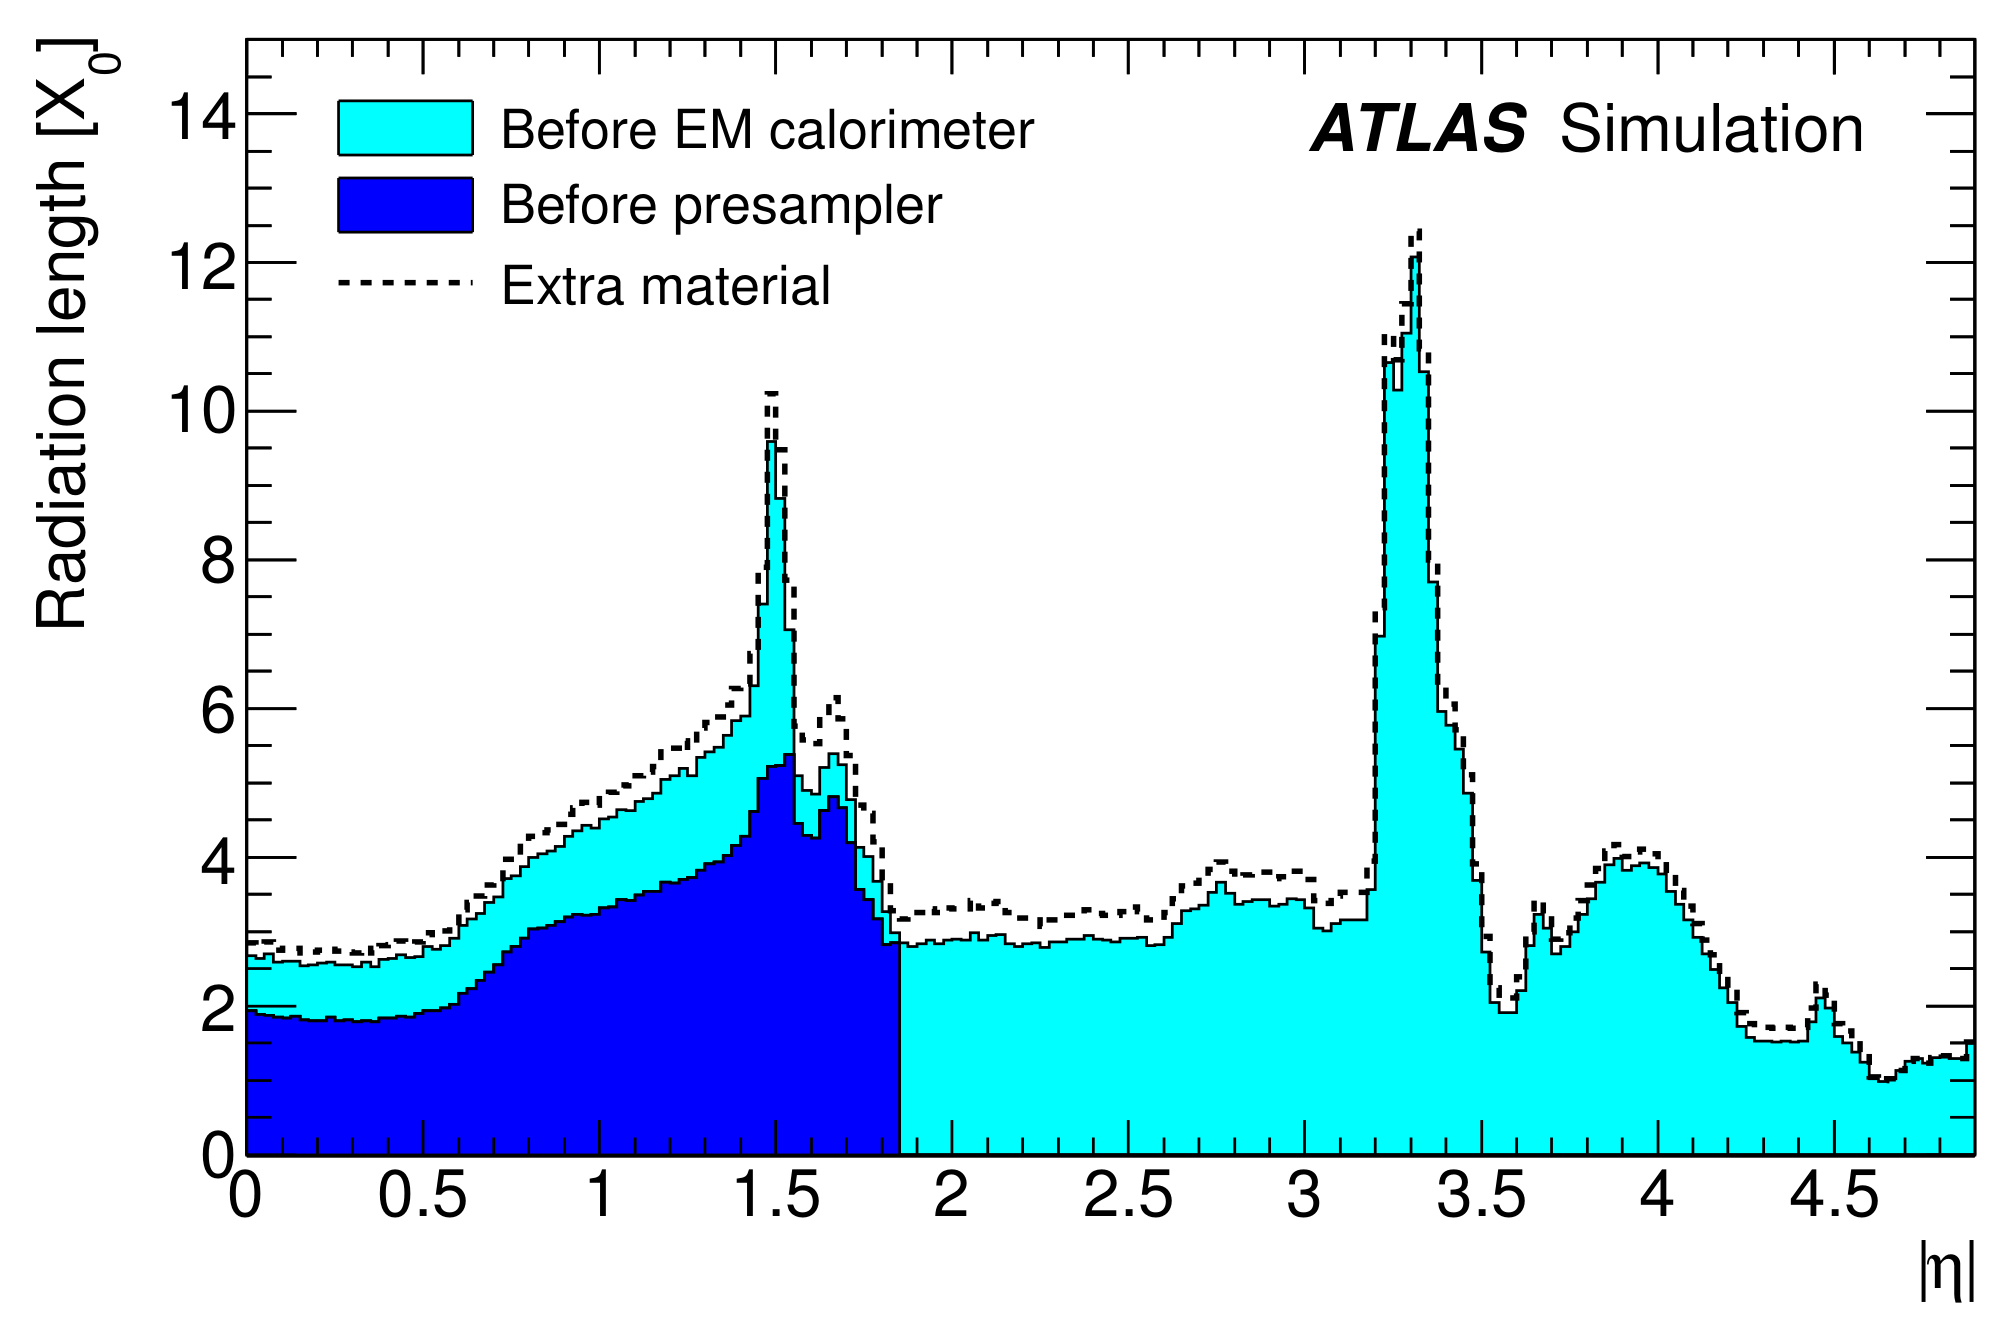
\includegraphics[width=0.7\textwidth]{img/extra_material}
    \caption[Material vor dem EM-Kalorimeter]
        {Die Menge an Material in Einheiten der Strahlungslänge $X_0$, die die
        Elektronen vor dem Kalorimeter durchfliegen, als Funktion der 
        Pseudorapidität $\eta$. Das zusätzliche Material wurde hier lediglich 
        zu systematischen Studien eingeführt und entspricht nicht der 
        tatsächlichen Verteilung. (Quelle: \cite{Aad:2011mk})}
    \label{fig:extra_material}
\end{figure}

Eine zusätzliche Unterteilung im Azimuthalwinkel $\phi$ wird nicht
vorgenommen, vielmehr geht man hier von einer isotropen Verteilung aus.
\newline

Wie bereits im einführenden Abschnitt \ref{energy_calibration:grundlagen}
erwähnt, werden die Elektronen im Zentral-Bereich als bereits perfekt
kalibriert angenommen, sodass gilt:
\begin{equation}
    \label{definition:perfect_central_electrons}
    E_\text{(data)}^\text{C} = E_\text{(MC)}^\text{C}
    \qquad \Longleftrightarrow \qquad
    \alpha_i^\text{C} = 0
    \qquad\qquad
    ^C : \text{zentral}
\end{equation}
Für die Messung der invarianten Masse (\ref{invariant_mass:basic}) des
\acs{CF}-Elektron-Paares folgt nun mit (\ref{definition:energy_scale}) und
(\ref{definition:perfect_central_electrons}):
\begin{align}
    m_\text{(data)}   &= \sqrt{ 2 \cdot E^C_\text{(data)} E^F_{\text{(data)}}
                         (1-\cos\theta)} 
                         \qquad ^C: \text{zentral}, \quad ^F: vorwärts
                         \nonumber \\[5pt]
                      &= \sqrt{ 2 \cdot E^C_\text{(MC)} E^F_{\text{(MC)}}
                         (1+\alpha^F_i)(1-\cos\theta)}
                         \nonumber \\[15pt]
    m^2_\text{(data)} &= 2 \cdot E^C_\text{(MC)} E^F_{\text{(MC)}}
                         (1+\alpha^F_i)(1-\cos\theta)
                         \nonumber \\[5pt]
                      &= m^2_\text{(MC)} (1+\alpha^F_i)
                         \label{eq:invariant_mass_sq}
\end{align}
Gleichung (\ref{eq:invariant_mass_sq}) liefert somit die Möglichkeit zur
Extraktion der Kalibrations-Faktoren
\begin{equation}
    \label{eq:extraction_alpha}
    \alpha_i^F = \frac{m^2_\text{(data)}}{m^2_\text{(MC)}} - 1
\end{equation}

Neben der der Korrektur der Energieskala in Daten, muss auf Seiten der
Simulation noch die Energieauflösung\footnote{siehe hierzu auch Kapitel
\ref{experimenteller_aufbau:atlas_detector:elektromagnetisches_kalorimeter}}
korrigiert werden. Wie eingangs bereits erwähnt ist die Auflösung des
Kalorimeters in der Simulation oftmals überschätzt, sodass eine zusätzliche
künstliche Verschmierung eingeführt wird um dies zu kompensieren.

Nach Gleichung (\ref{eq:calorimeter_resolution}) ist die Auflösung des
Kalorimeters gegeben durch 
\begin{equation}
    \left(\frac{\sigma_E}{E}\right)_\text{(MC)} =
        \frac{a}{\sqrt{E}} \oplus \frac{b}{E} \oplus c
\end{equation}
Der sognannte \textit{Sampling Term} $a$ wird dabei als von der Simulation
wohl modelliert angenommen, während der \textit{Rauschterm} $b$ aus Messungen
mit Test-Strahlen extrahiert wird (siehe \cite{1748-0221-5-11-P11006}). Jeder
zusätzliche Beitrag spiegelt sich im konstanten Term $c$ wieder. Dieser ist
nicht simulierbar und muss aus einem Vergleich mit der tatsächlichen Auflösung
in den Daten gewonnen werden. Dazu bildet man die partiellen Ableitungen von
Gleichung (\ref{invariant_mass:basic})
\begin{align}
    \frac{\del m}{\del E_i} \;&=\; \frac{1}{2m} \frac{m^2}{E_i}
        \;=\; \frac{m}{2 E_i} \qquad\quad i \in \{1,2\}
\end{align}
und bildet die Gaußsche Fehlerfortpflanzung für die Auflösung der invarianten
Masse:
\begin{align}
    \sigma_m^2 \;&=\; \left(\frac{\del m}{\del E_1}\sigma_{E_1}\right)^2 +
                      \left(\frac{\del m}{\del E_2}\sigma_{E_2}\right)^2
                \;=\; \frac{m^2}{4E_1^2}\sigma_{E_1}^2 +
                      \frac{m^2}{4E_2^2}\sigma_{E_2}^2
                      \nonumber \\[5pt]
    \Longleftrightarrow \quad
    \frac{4\sigma_m^2}{m^2} &= \frac{\sigma_{E_1}^2}{E_1^2} +
                               \frac{\sigma_{E_2}^2}{E_2^2}
\end{align}
Führt man nun für die Auflösung in der Simulation den konstanten Term $c$ ein
und vergleicht mit der Auflösung in den Daten so folgt:
\begin{align}
    &\sigma_{E_i}^2/E_i^2 \longrightarrow \sigma_{E_i}^2/E_i^2 + c_i^2
    \nonumber \\[10pt]
    &4\left(\frac{\sigma_m^2}{m^2}\right)_\text{(data)}
        = 4\left(\frac{\sigma_m^2}{m^2}\right)_\text{(MC)}
        + c_1^2 + c_2^2
\end{align}
Auch hier wird, wie schon bei der Energieskala, die Kalibration der
Zentral-Elektronen als perfekt angenommen, sodass $c_1 = 0$ gesetzt werden
kann. Desweiteren wird ebenfalls eine Unterteilung des Kalorimeters in der
Pseudorapidität $\eta$ vorgenommen\footnote{Es handelt sich um die selbe
Unterteilung, wie schon für die Kalibrations-Faktoren der Energieskala},
was durch den Index $i$ angezeigt wird.
\begin{align}
    \label{eq:extraction_constant_terms}
    4\left(\frac{\sigma_m^2}{m^2}\right)_\text{(data)}
        &= 4\left(\frac{\sigma_m^2}{m^2}\right)_\text{(MC)}
        + \left(c_i^F\right)^2
\end{align}
Gleichung (\ref{eq:extraction_constant_terms}) bietet somit die Möglichkeit zur
Extraktion der Verschmierungsterme
\begin{align}
    c_i^F &= \sqrt{ 4 \left[ \left(\frac{\sigma_m}{m}\right)^2_\text{(data)}
             - \left(\frac{\sigma_m}{m}\right)^2_\text{(MC)} \right] }
    \label{eq:constant_terms}
\end{align}



\subsection{Extraktionsmethode}
\label{energy_calibration:extraktionsmethode}
Nachdem nun die notwendigen Definitionen und Annahmen zur Exktraktion der
Kali\-brations-Faktoren getroffen wurden, kann eine Prozedur zu deren
Bestimmung entwickelt werden.

Es müssen die Energieskalen\footnote{Der obere Index $F$ an den
Kalibrations-Faktoren wird hier und im Folgenden der Einfachheit halber
weggelassen} $\alpha_i$ und die Verschmierungsterme $c_i$ für jeden Bereich in
$\eta$ separat gewonnen werden. Angepasst an die typischen Größen der
Elektronschauer\footnote{vlg hierzu auch Kapitel
\ref{experimenteller_aufbau:elektronen_in_atlas}} im Kalorimeter hat sich
folgene Unterteilung in der Pseudorapidität als sinnvoll erwiesen:

\begin{table}[h]
    \centering
    \begin{tabular}{|c|c|c|c|c|c|}
        \multicolumn{6}{c}{\textbf{EMEC}} \\
        \hline
        2.5 - 2.6 & 2.6 - 2.7 & 2.7 - 2.8 & 2.8 - 2.9 & 2.9 - 3.0 & 3.0 - 3.16
        \\ \hline
    \end{tabular}
    \vspace{10pt}

    \begin{tabular}{|c|c|c|}
        \multicolumn{3}{c}{\textbf{FCal}} \\
        \hline
        3.35 - 3.6 & 3.6 - 4.0 & 4.0 - 4.9 \\
        \hline
    \end{tabular}
    \caption{Unterteilung der Vorwärts-Kalorimeter in der Pseudorapidität
             $|\eta|$ zur Extraktion der Kalibrations-Konstanten}
    \label{tab:calibration_binning}
\end{table}

Der Bereich zwischen $3.16 < |\eta| < 3.35$ wurde exkludiert, da sich
hier der Übergangsbereich zwischen \acs{EMEC} und \acs{FCal} befindet.

Das grundlegende Prinzip zur Extraktion der Kalibrations-Faktoren besteht nun
darin, für jede Unterteilung des Kalorimeters (Tabelle
\ref{tab:calibration_binning}) die invarianten Massenspektren in Daten und
Simulation zu erstellen und mittels einer Kurvenanpassung analytischer
Funktionen die Parameter Masse und Auflösung für die Gleichungen
(\ref{eq:extraction_alpha}) und (\ref{eq:constant_terms}) zu bestimmen.

Zur Erstellung der invarianten Massenspektren werden Selektions-Schnitte
angewendet, die auf Seiten der Daten für eine Unterdrückung des Untergrundes
sorgen. Tabelle \ref{tab:calibration_cuts} zeigt eine Übersicht über die
verwendeten Schnitte\footnote{Eine detailiertere Beschreibung der Schnitte
findet sich in Kapitel \ref{daten_simulation_selektion:selektion}} auf Daten
und Simulation.

\begin{savenotes}
\begin{table}[h]
    \centering
    \begin{tabular}{|c|c|}
        \hline
        \multicolumn{2}{|c|}{\textbf{Event basierte Schnitte}} \\
        \hline\hline
        \acs{GRL} (nur Daten) & (...)\_EgammaForward.xml\footnote{Verwendete
            \ac{GRL}:
            data12\_8TeV.periodAllYear\_DetStatus-v61-pro14-02
            \_DQDefects-00-01-00\_PHYS\_StandardGRL\_All\_Good
            \_EgammaForward.xml} \\
        \hline
        Trigger & e24vhi\_medium1 \textit{or} e60\_medium1 \\
        \hline
        primärer Vertex & $\geq 3$ \\
        \hline
    \end{tabular}
    \vspace{15pt}

    \begin{tabular}{|c|c|c|}
        \hline
        \multicolumn{3}{|c|}{\textbf{Elektron basierte Schnitte}} \\
        \textbf{Schnitt}&\textbf{Zentral-Elektron}&\textbf{Vorwärts-Elektron}\\
        \hline \hline
        Pseudorapidität & $|\eta| \leq 2.47$ & $2.5 \leq |\eta| \leq 4.9$ \\
        \hline
        Transversal-Impuls & $p_T > 25.0 \GeV$ & $p_T > 20.0 \GeV$ \\
        \hline
        Autor & 1 \textit{or} 3 & 8 \\
        \hline
        ID & \textit{tight++} & \textit{forward\_tight} \\
        \hline
        OQ & \multicolumn{2}{|c|}{- good object quality -} \\
        \hline
    \end{tabular}
    \caption{Übersicht über die bei der Energiekalibration verwendeten
        Selektions-Schnitte auf Daten und Simulation}
    \label{tab:calibration_cuts}
\end{table}
\end{savenotes}

Für die Kurvenanpassung wird zur Beschreibung des Signal-Anteils die aus der
theoretischen Vorhersage bekannte Breit-Wigner-Verteilung\footnote{siehe
\cite{PhysRev.49.519}} für die Z-Resonanz benutzt. Um die endliche Auflösung
des Detektors sowie Bremsstrahlungseffekte der Elektronen zu berücksichtigen,
wird diese Verteilung mit einer Crystal-Ball Distribution\footnote{siehe
\cite[Appendix F]{Gaiser:1982yw}} gefaltet. Diese besteht aus einer Gaußschen
Glockenkurve zur Beschreibung der Auflösung und geht links des Maximums in
einen langsam Abfallenden Polynomischen Anteil über, der die Verschiebung zu
niederigeren invarianten Massen durch Bremsstrahlung repräsentiert (siehe
Abbildung \ref{fig:crystal_ball}, rechts). Die analytische Form beider
Verteilungen zeigen die Gleichungen (\ref{eq:breit_wigner}) und
(\ref{eq:crystal_ball}) 
\begin{align}
    f_\text{BW}(x) &= \frac{1}{(x-\mu)^2+\frac{1}{4}\sigma^2}
    \label{eq:breit_wigner}\\[10pt]
    f_\text{CB}(x) &=
        \begin{cases}
            \frac{(\frac{n}{|\alpha|})^n e^{-\frac{1}{2}\alpha^2}}
                 {\left( \frac{n}{|\alpha|}-|\alpha|-x \right)^n}
                & \text{,für}\quad x < -|\alpha| \\
            \exp\Bigl[-\frac{1}{2}\left( \frac{x-\mu}{\sigma} \right)^2 \Bigr]
                & \text{,für}\quad x > -|\alpha|
        \end{cases}
    \label{eq:crystal_ball}
\end{align}

\begin{figure}
    \centering
    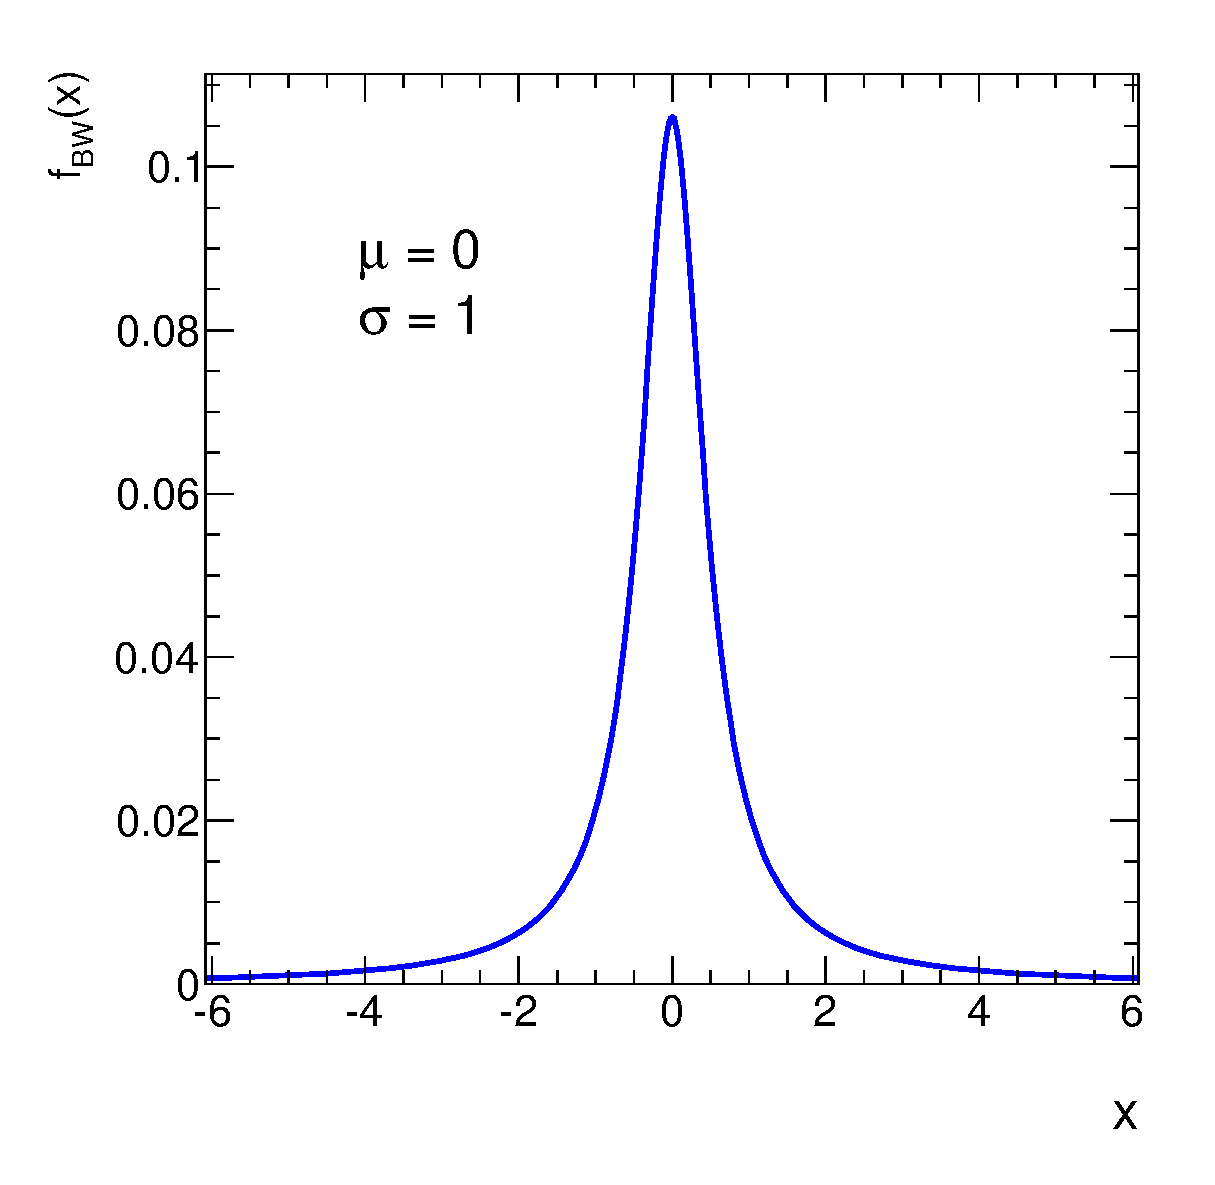
\includegraphics[width=0.48\textwidth]{plots/breit_wigner}
    \hfill
    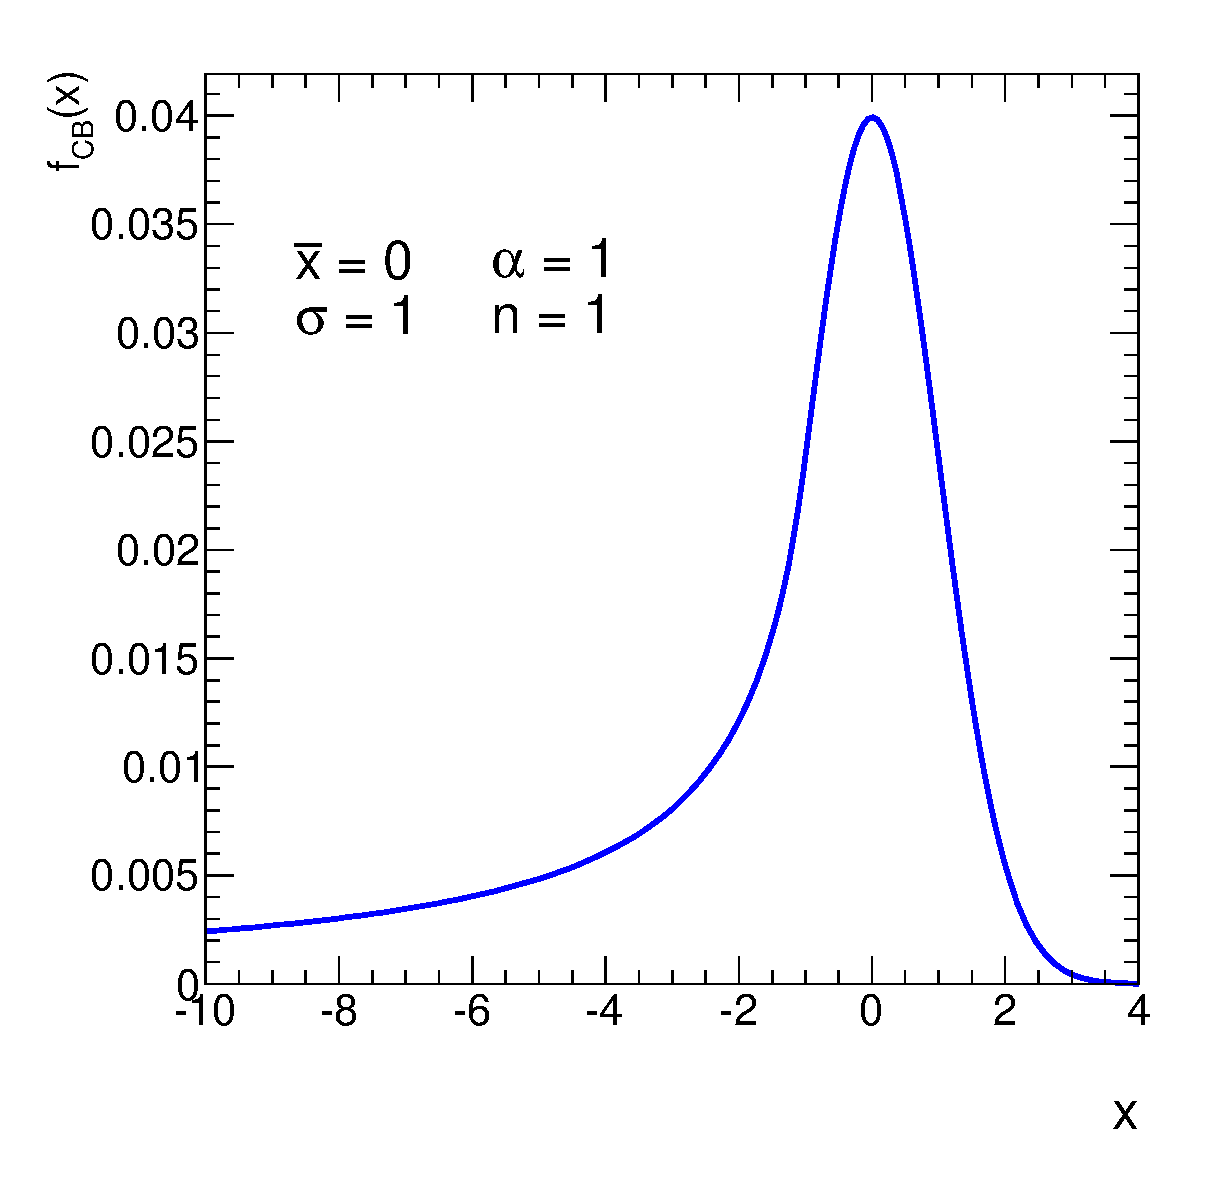
\includegraphics[width=0.48\textwidth]{plots/crystal_ball}
    \caption[Wahrscheinlichkeitsdichte-Verteilungen für eine Breit-Wigner
        Verteilung und eine Crystal-Ball Verteilung]
        {Wahrscheinlichkeitsdichte-Verteilungen für eine Breit-Wigner
        Verteilung (links) und eine Crystal-Ball Verteilung (rechts) mit
        illustrativ gewählten Parametern}
    \label{fig:crystal_ball}
\end{figure}

Die Faltung beider Verteilungen dient zur Beschreibung des Signals und wird in
den Spektren der Simulation zur Kurvenanpassung verwendet.
\begin{equation}
    f_\text{sig}(m_{ee}) = f_\text{BW}(m_{ee}) \;\otimes\; f_\text{CB}(m_{ee})
    \label{eq:fit_model}
\end{equation}
Zur Anpassung an die Datenverteilungen muss die obige Gleichung
(\ref{eq:fit_model}) noch um einen weiteren Term erweitert werden, um den nach
Selektion noch verbleibenden Untergrund abzuschätzen. Hierfür wird eine
exponentiel abfallende Verteilung benutzt:
\begin{equation}
    f_\text{sig+bkg}(m_{ee}) = f_\text{BW}(m_{ee})
        \;\otimes\; f_\text{CB}(m_{ee})
        \;+\; f_\text{exp}(m_{ee})
    \label{eq:fit_model_bkg}
\end{equation}

Die für die Extraktion den Kalibration-Faktoren relevanten Parameter des
Modells sind der Erwartungswert der Breit-Wigner-Verteilung $\mu_\text{BW}$,
der die Position der Resonanz beschreibt und somit die Energieskala
determiniert, sowie die Breite der Crystal-Ball-Verteilung $\sigma_\text{CB}$,
welche die Detektorauflösung repräsentiert. Die jeweils korrespondierenden
Parameter, also der Erwartungswert Crystal-Ball-Verteilung $\mu_\text{CB}$ und
die Breite der Breit-Wigner-Verteilung $\sigma_\text{BW}$, werden während der
Kurvenanpassung konstant gehalten, um Interferenzen mit den relevanten
Parametern zu umgehen. Die Wahl der festen Parameter ist in Tabelle
\ref{tab:fit_parameters} zu finden, wobei der Wert für $\sigma_{BW}$ auf die
Breite des Z-Resonanz gesetzt wurde (siehe \cite{PhysRevD.86.010001})

\begin{table}[h]
    \centering
    \begin{tabular}{|l|c|c|}
        \hline
        \textbf{Verteilung} & \textbf{Parameter} & \textbf{Wert} \\
        \hline \hline
        \multirow{2}{*}{Breit-Wigner} & $\mu_\text{BW}$      & frei       \\
                                      & $\sigma_\text{BW}$   & $2.49\GeV$ \\
        \hline
        \multirow{4}{*}{Crystal-Ball} & $\mu_\text{CB}$      & $0.00\GeV$ \\
                                      & $\sigma_\text{CB}$   & frei       \\
                                      & $\alpha_\text{CB}$   & frei       \\
                                      & $n_\text{CB}$        & frei       \\
        \hline
        Exponential (nur in Daten)    & $\alpha_\text{exp}$  & frei       \\
        \hline
    \end{tabular}
    \caption{Übersicht der Parameter für Kurvenanpassungen in invarianten
        Massenspektren zur Energiekalibration}
    \label{tab:fit_parameters}
\end{table}

Die tatsächliche Prozedur zur Extraktion der Kalibrations-Faktoren ist
mehrstufig aufgebaut und lässt sich iterativ beschreiben:
\begin{description}
    \item[Vorbereitung I:]
        Selektion der Daten und Simulations-Ereignisse mit Anwendung der
        Kalibration-Faktoren für Zentral-Elektronen.
    \item[Extraktion I:]
        Erstellung der invarianten Massenspektren und Durchführung der
        Kurvenanpassung. Extraktion der Kalibration-Faktoren $\alpha_i$ der
        Energieskala aus den Parametern $\mu_\text{BW}$ der Kurvenanpassung
        mittels Gleichung (\ref{eq:extraction_alpha}).
    \item[Vorbereitung II:]
        Selektion der Daten und Simulations-Ereignisse mit Anwendung der
        Kalibration-Faktoren für Zentral-Elektronen und der neu gewonnen
        Energieskalen $\alpha_i$ für Vorwärts-Elektronen in Daten.
    \item[Extraktion II:]
        Erstellung der invarianten Massenspektren und Durchführung der
        Kurvenanpassung. Extraktion der Kalibration-Faktoren $c_i$ der
        Auflösung aus den Parametern $\mu_\text{BW}$ und $\sigma_{CB}$ der
        Kurvenanpassung mittels Gleichung (\ref{eq:constant_terms}).
\end{description}
Die Kalibration-Faktoren $\alpha_i$ und $c_i$ können mit dem hier gewählten
Ansatz der Extraktion\footnote{Andere Möglichkeiten zur Extraktion der
Kalibrationskonstanten werden im abschließenden Abschnitt
\ref{energy_calibration:ergebnisse_und_ausblick} diskutiert} aus den Parametern
von Kurvenanpassungen nicht simultan in einem Schritt extrahiert werden, da
Gleichung (\ref{eq:constant_terms}) unmittelbar von der Energieskala abhängt
und somit die oben beschriebene Mehrstufigkeit indiziert.



%______________________________________________________________________________
%                                       Exktraktion der Kalibrations-Konstanten
%
\section{Extraktion der Kalibrations-Konstanten}
\label{energy_calibration:extraktion_der_kalibrations-konstanten}

\begin{itemize}
    \item \sout{Beispielhafte Fits}
    \item \sout{Effizienzkurve}
    \item \sout{Exktraktion der Energy-Scales}
    \item \sout{Extraktion der Constant-Terms}
    \item \sout{Closure-Tests}
    \item Systematiken
\end{itemize}

Der Kalibration zugrunde liegen der volle Datensatz aus 2012 mit $8\TeV$
Schwer\-punktsenergie und einer integrierten Gesamtluminosität\footnote{nach
Anwendung der \ac{GRL}} von $20.3\fb^{-1}$, sowie simulationsseitig das
inklusiv in der invarianten Masse generierte $Z\rightarrow ee$
Signal-Monte-Carlo\footnote{Dataset ID: 147806 (siehe Tabelle
\ref{tab:MC_samples})} mit etwa 10 Millionen generierten Ereignissen. Nach
Anwendung der Selektions-Kriterien (Tabelle \ref{tab:calibration_cuts})
verbleiben noch 4577323 Ereignisse ($\approx 12\%$) in Daten und 949095
Ereignisse ($\approx 1\%$) in der Simulation. Tabelle
\ref{tab:remaining_electrons} zeigt eine detailiertere Darstellung über Anzahl
der Elektronkandidaten nach jedem Schnitt.

\begin{table}[h]
    \centering
    \begin{tabular}{|l|r|r|}
        \hline
        & \multicolumn{2}{|c|}{Elektronkandidaten} \\
        \textbf{Schnitt} & \textbf{Daten} & \textbf{Simulation} \\
        \hline\hline
        \ac{GRL}           & 3954702112 & (75195428) \\
        Detektor Status    & 3945153030 & (75195428) \\
        Trigger            & 1402546381 & 48781893 \\
        primärer Vertex    & 1400899527 & 48503958 \\
        Pseudorapidität    & 1328016208 & 46608879 \\
        Transversal-Impuls &  498956943 & 19742239 \\
        Autor              &  378463236 & 18690503 \\
        ID                 &   76603185 &  9441601 \\
        OQ                 &   75178238 &  9263740 \\
        \hline
    \end{tabular}
    \caption[Anzahl der Elektronkandidaten in Simulation und Daten nach
        Selektionschnitten]
        {Anzahl der Elektronkandidaten in Simulation und Daten nach
        Selektionschnitten. Die Auflistung ist inklusiv, d.h. untere Schnitte
        enthalten implizit alle vorangegangenen Schnitte. \textit{\ac{GRL}} und
    \textit{Detektor Status} sind für Simulationsergeignisse irrelevant.}
    \label{tab:remaining_electrons}
\end{table}

Die invarianten Massenspektren werden nun aus den Ereignissen erstellt, die
alle Schnitte passieren konnten, und werden standardmäßig in einem Fenster
zwischen $75 \GeV$ und $105 \GeV$ betrachtet. In simulierte Spektren gehen die
Monte-Carlo-Ereignisse dabei stets mit einem individuellen Gewicht in die
Histogramme ein. Die Zusammensetzung der Gewichte 
\begin{equation}
    w_\text{event} = w_\text{pile-up} \cdot w_\text{vertex-pos} \cdot
                     w_\text{ID} \cdot w_\text{reco} \cdot w_\text{trigger}
    \label{eq:calibration_weights}
\end{equation}
beinhaltet Korrekturen für ungleiche Pile-Up Bedingungen, die Position des
Primärvertex, sowie unterschiedliche Effizienzen bei der Rekonstruktion,
Identifikation und Triggersimulation der Elektronen\footnote{mehr zu Grundlagen
und Anwendung der verwendeten Gewichte in Kapitel
\ref{daten_simulation_selektion:korrekturen}}.

Abbildung \ref{fig:example_mee_p26} zeigt beispielhaft zwei resultierende
Massenspektren aus Daten und Simulation.

\begin{figure}
    \centering
    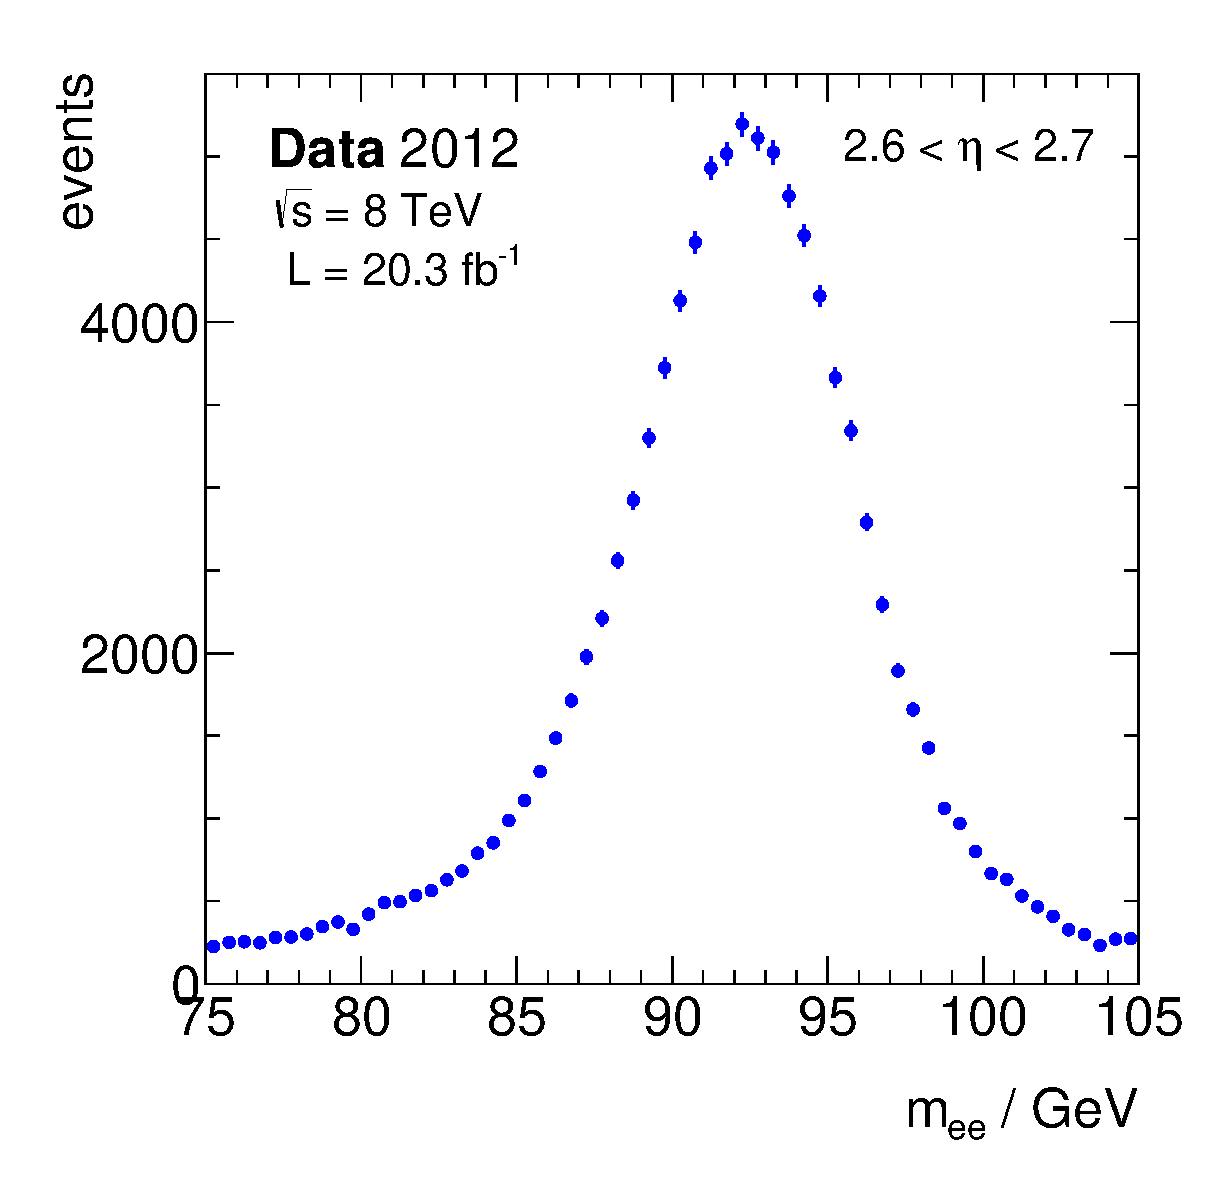
\includegraphics[width=0.48\textwidth]{plots/example_mee_data_p26}
    \hfill
    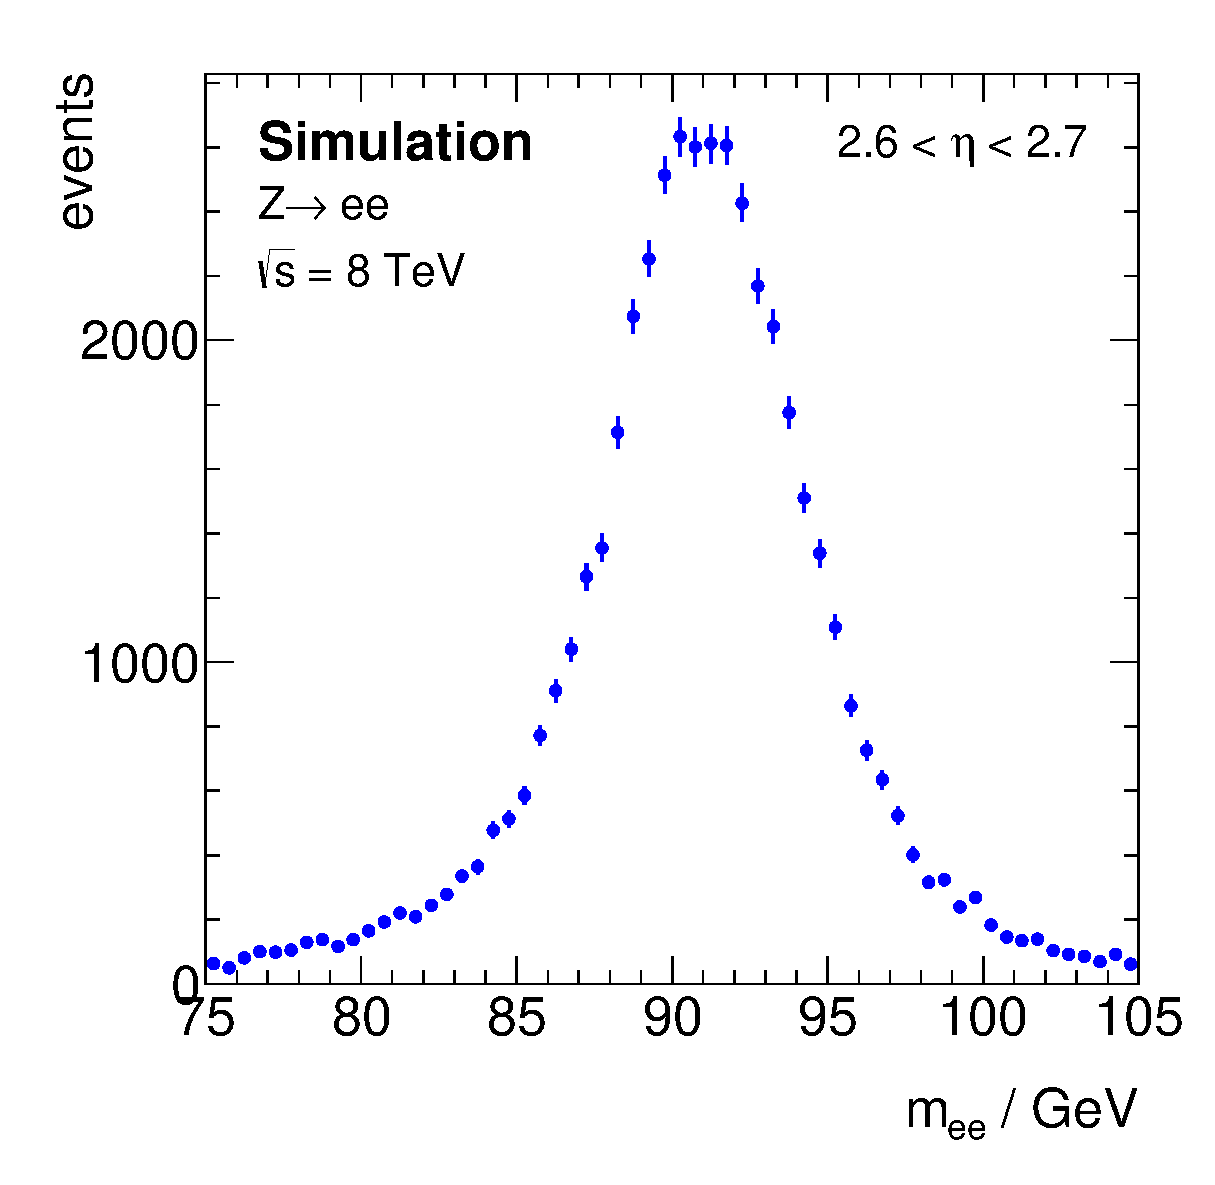
\includegraphics[width=0.48\textwidth]{plots/example_mee_mc_p26}
    \caption[Beispielhafte invariante Massenspektren nach Selektion aus Daten
        und Simulation für den Bereich $2.6 < \eta < 2.7$ der Pseudorapidität]
        {Beispielhafte invariante Massenspektren nach Selektion aus Daten
        (links) und Simulation (rechts) für den Bereich $2.6 < \eta < 2.7$ der
            Pseudorapidität.(Nur statistische Unsicherheiten)}
    \label{fig:example_mee_p26}
\end{figure}

Für die Kurvenanpassung wird das von W. Verkerke, D. Kirkby entwickelte
\textit{\textsc{RooFit} Paket für Datenmodellierung} (\cite{Verkerke:2003ir})
verwendet, dass bereits als \textsc{C++}-Bibliothek in \textsc{ROOT} zur
Verfügung steht und native Implementationen aller benötigten Verteilungen aus
(\ref{eq:fit_model}) bzw. (\ref{eq:fit_model_bkg}) bereit stellt.



\subsection{Erweiterung der Modelle und Extraktions-Prozedur}
\label{energy_calibration:erweiterung_der_modelle_und_prozedur}
Die simple Durchführung der Kurvenanpassung mit den oben beschriebenen Modellen
wirft allerdings zunächst zwei Probleme auf.

Zum einen hängen die Werte der resultierenden Parameter stark davon ab, welcher
Satz von Startparametern an die Minimierungsprozedur übergeben wird, da diese
häufig vor erreichen des globalen Minimums in lokale Minima konvergiert. Zur
Umgehung dieses Problems wird deshalb jede Kurvenanpassung 1000 mal
durchgeführt, wobei jedesmal ein anderer, zufällig innerhalb bestimmter Grenzen
generierter Satz von Parametern als Startwerte vorgegeben wird. Aus den dadurch
erzeugten 1000 Sätzen von resultierenden Parametern wird dann derjenige
ausgewählt, der die beste Beschreibung der Datenpunkte, quantifiziert über
einen $\chi^2$-Test, durch die analytischen Funktionen liefert.

Zum anderen führt die Wahl der Schnitte auf die Transversal-Impulse in
Kombination mit einem durch die \ac{CF}-Selektion determinierten Öffnungswinkel
der Elektronen zu einer Verzerrung der Form der Z-Resonanz, insbesondere für
hohe Pseudorapiditäten des Vorwärts-Elektrons. Dies hat zur Folge, dass der
Bereich des invarianten Massenspektrums links der Resonanz deutlich weniger
populiert ist, als es die analytischen Modelle (\ref{eq:fit_model}) und
(\ref{eq:fit_model_bkg}) zu beschreiben in der Lage sind. Abbildung
\ref{fig:example_fits} zeigt die Kurvenanpassung von Gleichung
(\ref{eq:fit_model_bkg}) an die Daten und Simulation in für einen nah an der
Strahlachse liegenden Bereich des Kalorimeters.

\begin{figure}
    \centering
    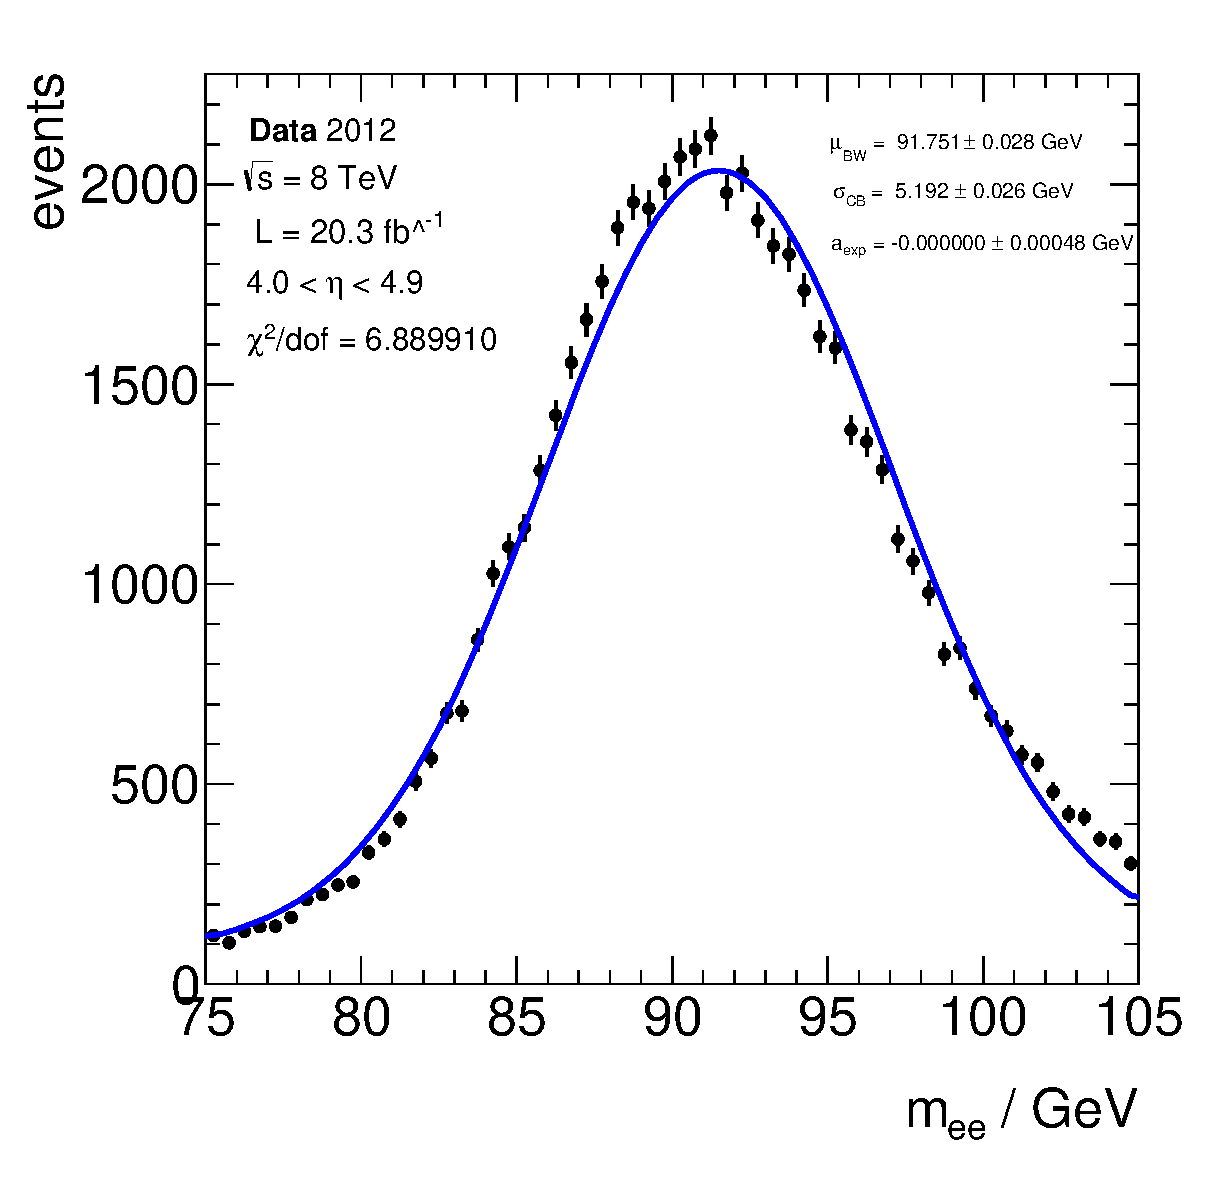
\includegraphics[width=0.48\textwidth]{plots/bad_fit_data_p40}
    \hfill
    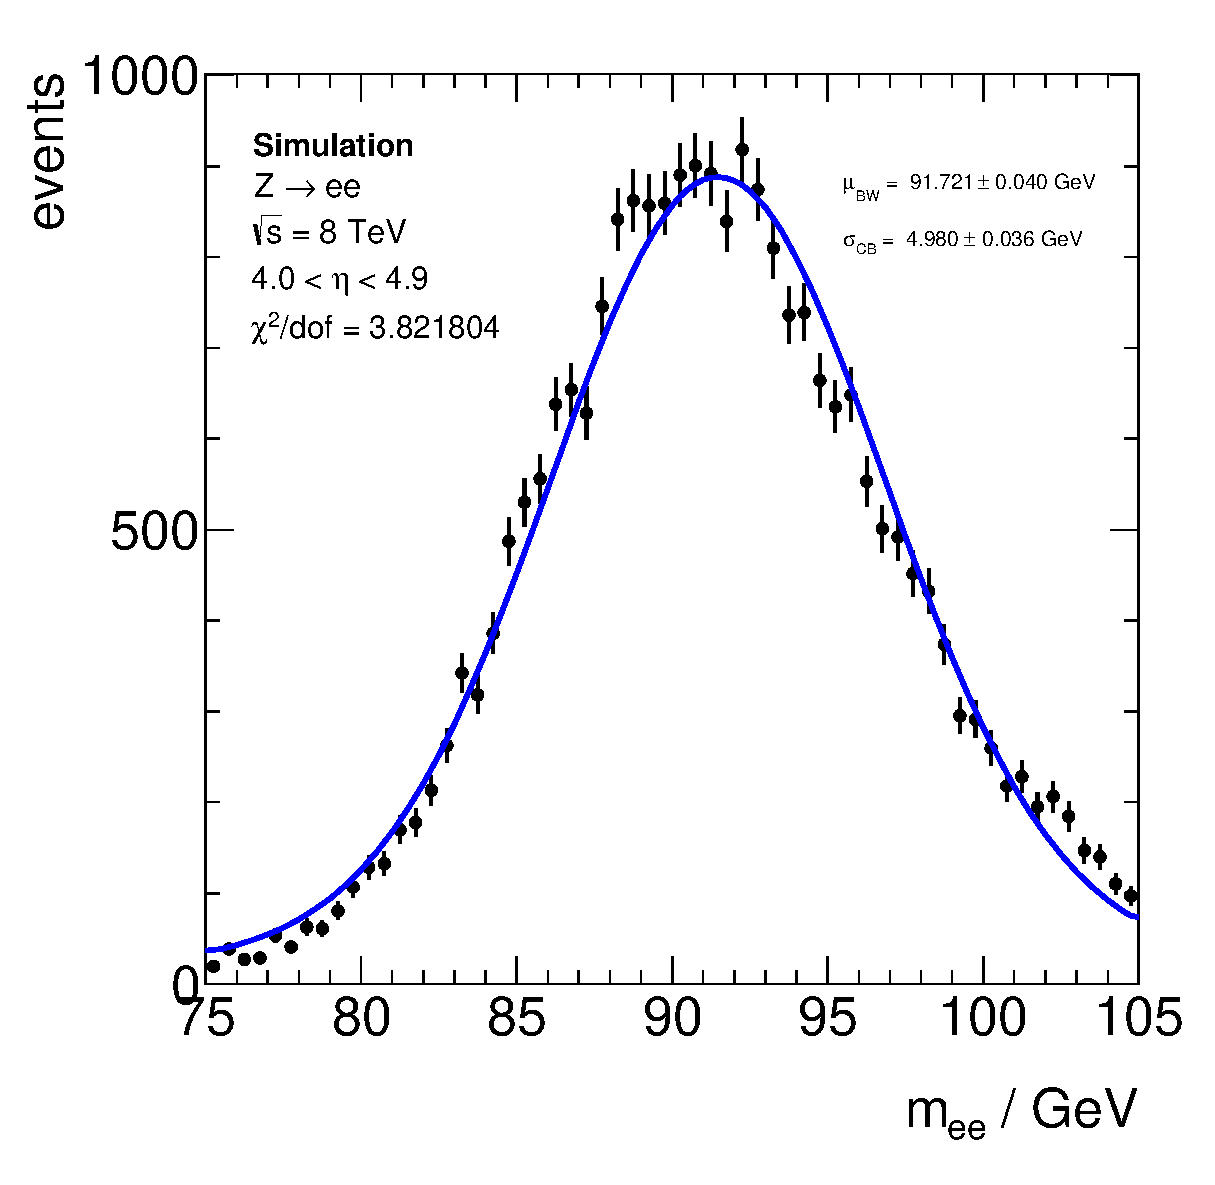
\includegraphics[width=0.48\textwidth]{plots/bad_fit_mc_p40}
    \caption[Kurvenanpassung ohne Berücksichtigung der Verzerrung der
        Z-Resonanz durch die kinematischen Schnitte]
        {Kurvenanpassung ohne Berücksichtigung der Verzerrung der Z-Resonanz
        durch die kinematischen Schnitte für den mittleren \acs{FCal}-Bereich
        in Daten (links) und Simulation (rechts)}
    \label{fig:example_fits}
\end{figure}

Die Lösung dieses Problems liegt in der Erweiterung der Modelle um eine weitere
Funktion, welche die oben beschriebene Verzerrung des Spektrums abbildet. Eine
Betrachtung der invarianten Massenverteilung der Elektronen auf Generator-Level
gibt Aufschluss über die Auswirkung der kinematischen Schnitte ohne die
Beeinflussung durch Detektoreffekte zu implizieren. Abbildung
\ref{fig:efficiency_p40} zeigt für den selben Bereich des Kalorimeters das
Verhältnis des invarianten Massenspektrum auf Generator-Niveau mit und ohne
kinematische Schnitte. Die Indizes $p_T,\eta$ am Dividenden symbolisiert die
Anwendung der Schnitte auf Transversal-Impuls und Pseudorapidität.

\begin{figure}
    \centering
    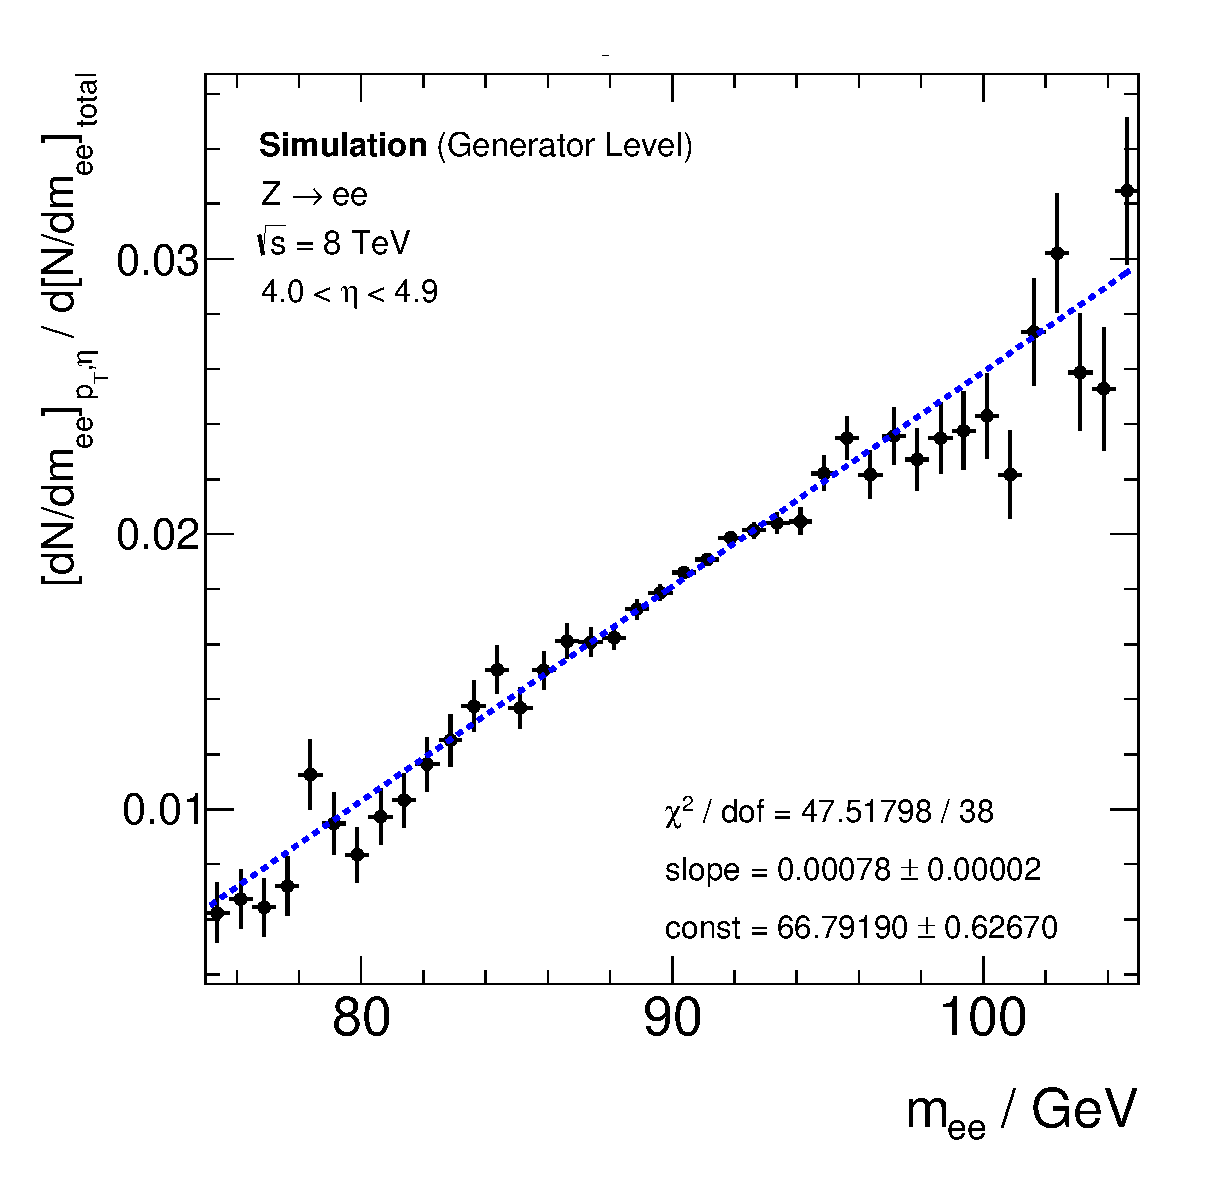
\includegraphics[width=0.6\textwidth]{plots/efficiency_p40}
    \caption[Quotient der invarianten Massenspektren mit und ohne kinematische
        Schnitte auf Generator-Level]
        {Quotient der invarianten Massenspektren mit und ohne kinematische
        Schnitte auf Generator-Level (schwarz). Kurvenanpassung einer linearen
        Funktion (blau).}
    \label{fig:efficiency_p40}
\end{figure}

Wie sich zeigt weist dieser Quotient, im Folgenden mit \textit{kinematischer
Akzeptanz} bezeichnet, einem linearen Verlauf, was die Modellierung durch
folgende Funktion nahe legt:
\begin{equation}
    f_\text{acc}(m_{ee}) = s \cdot (m_{ee}-c)
    \label{eq:acceptance}
\end{equation}
Alle anderen Bereiche der Vorwärts-Kalorimeter zeigen einen ähnlichen linearen
Verlauf der Akzeptanz, sodass eine globale Erweiterung der analytischen Modelle
angestrebt werden kann:
\begin{equation}
    f_\text{sig(+bkg)}(m_{ee}) \longrightarrow f_\text{sig(+bkg)}(m_{ee})
    \cdot f_\text{acc}(m_{ee})
    \label{eq:fit_model_extended}
\end{equation}
Die Parameter $s$ und $c$ der Akzeptanz-Funktion werden dabei, wie bereits in
Abbildung \ref{fig:efficiency_p40} gezeigt, auf Generator-Level für jeden
Bereich des Kalorimeters separat bestimmt und während der eigentlichen
Kurvenanpassung von (\ref{eq:fit_model_extended}) zur Extraktion der
Kalibrations-Faktoren konstant gehalten, sodass durch die Erweiterung keine
zusätzlichen freien Parameter in die Modelle eingeführt werden. Tabelle
\ref{tab:acceptance_parameters} im Anhang zeigt eine Auflistung beider
Akzeptanzparameter für alle Bereiche.

Unter Berücksichtigung der kinematischen Akzeptanz verbessert sich die
Beschreibung der Datenpunkte durch die analytischen Modelle nach
Kurvenanpassung deutlich. Abbildung \ref{fig:good_example_fit} zeigt die
Kurvenanpassung im selben Bereich des Kalorimeters unter Einbeziehung der
kinematischen Akzeptanz Funktion in das Modell.

\begin{figure}
    \centering
    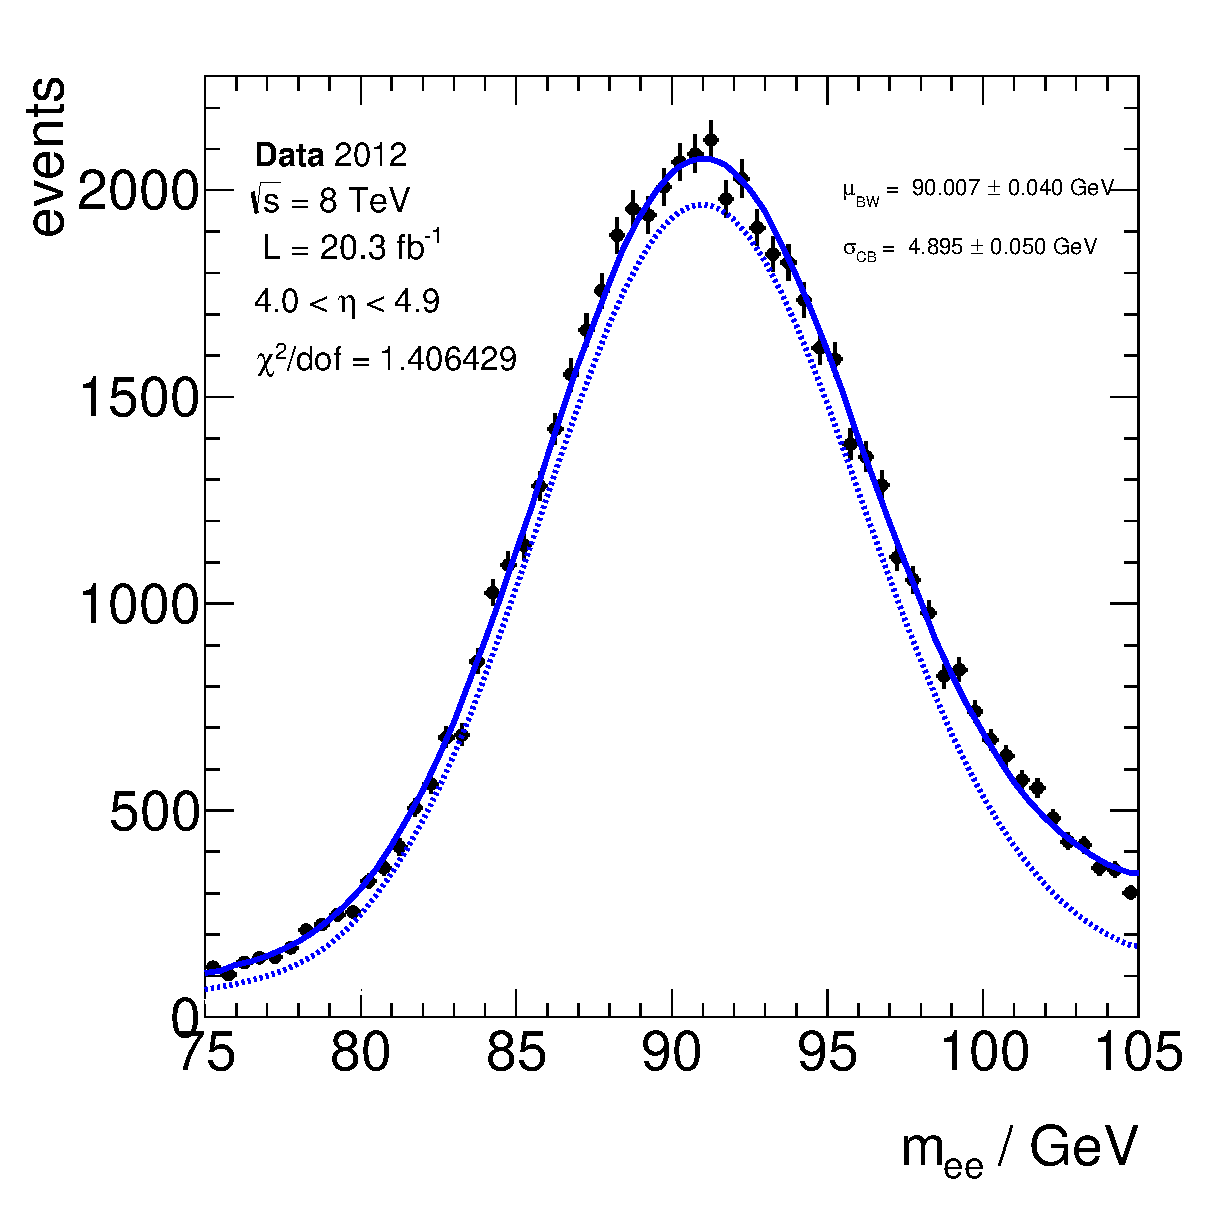
\includegraphics[width=0.48\textwidth]{plots/fit_data_p40}
    \hfill
    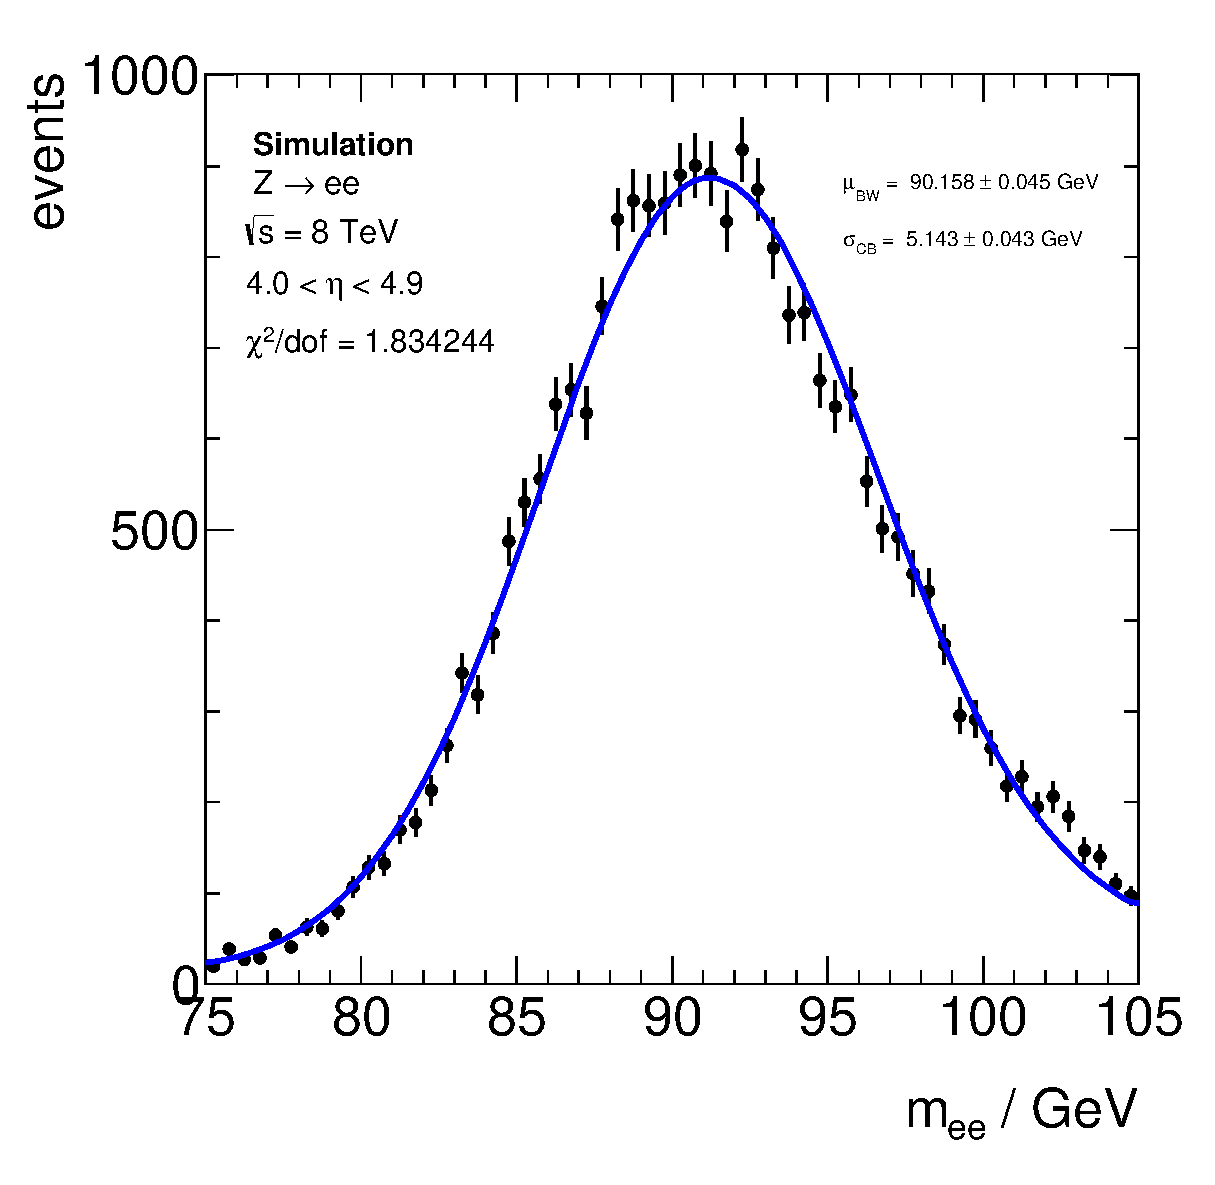
\includegraphics[width=0.5\textwidth]{plots/fit_mc_p40}
    \caption[Kurvenanpassung mit Berücksichtigung der kinematischen Akzeptanz]
        {Kurvenanpassung mit Berücksichtigung der kinematischen Akzeptanz für
        den mittleren \acs{FCal}-Bereich in Daten (links) und Simulation
        (rechts).}
    \label{fig:good_example_fit}
\end{figure}



\subsection{Extraktion der Kalibrations-Faktoren}
\label{energy_calibration:extraction_energy_scales}
Die Extraktion der Kalibrations-Faktoren der Energieskala basiert, wie in
Abschnitt \ref{energy_calibration:extraktionsmethode}
beschrieben, auf den selektierten Ereignissen mit kalibrierten
Zentral-Elektronen (\textit{Vorbereitung I}) und der eigentlichen Bestimmung
der Faktoren $\alpha_i$ aus den darauf folgenden Kurvenanpassungen
(\textit{Extraktion I}) der invarianten Massenspektren. In Abbildung
\ref{fig:alpha_stat} sind die resultierenden Werte der Kalibrationfaktoren
$\alpha_i$ dargestellt. Die angegebenen Unsicherheiten sind hier rein
statistischer Natur und resultieren aus der \textit{Schätzung} der Parameter
durch die Kurvenanpassung\footnote{Studien zu systematischen Variationen folgen
in Abschnitt \ref{energy_calibration:systematics}}.

\begin{figure}[h]
    \begin{minipage}{0.48\textwidth}
        \centering
        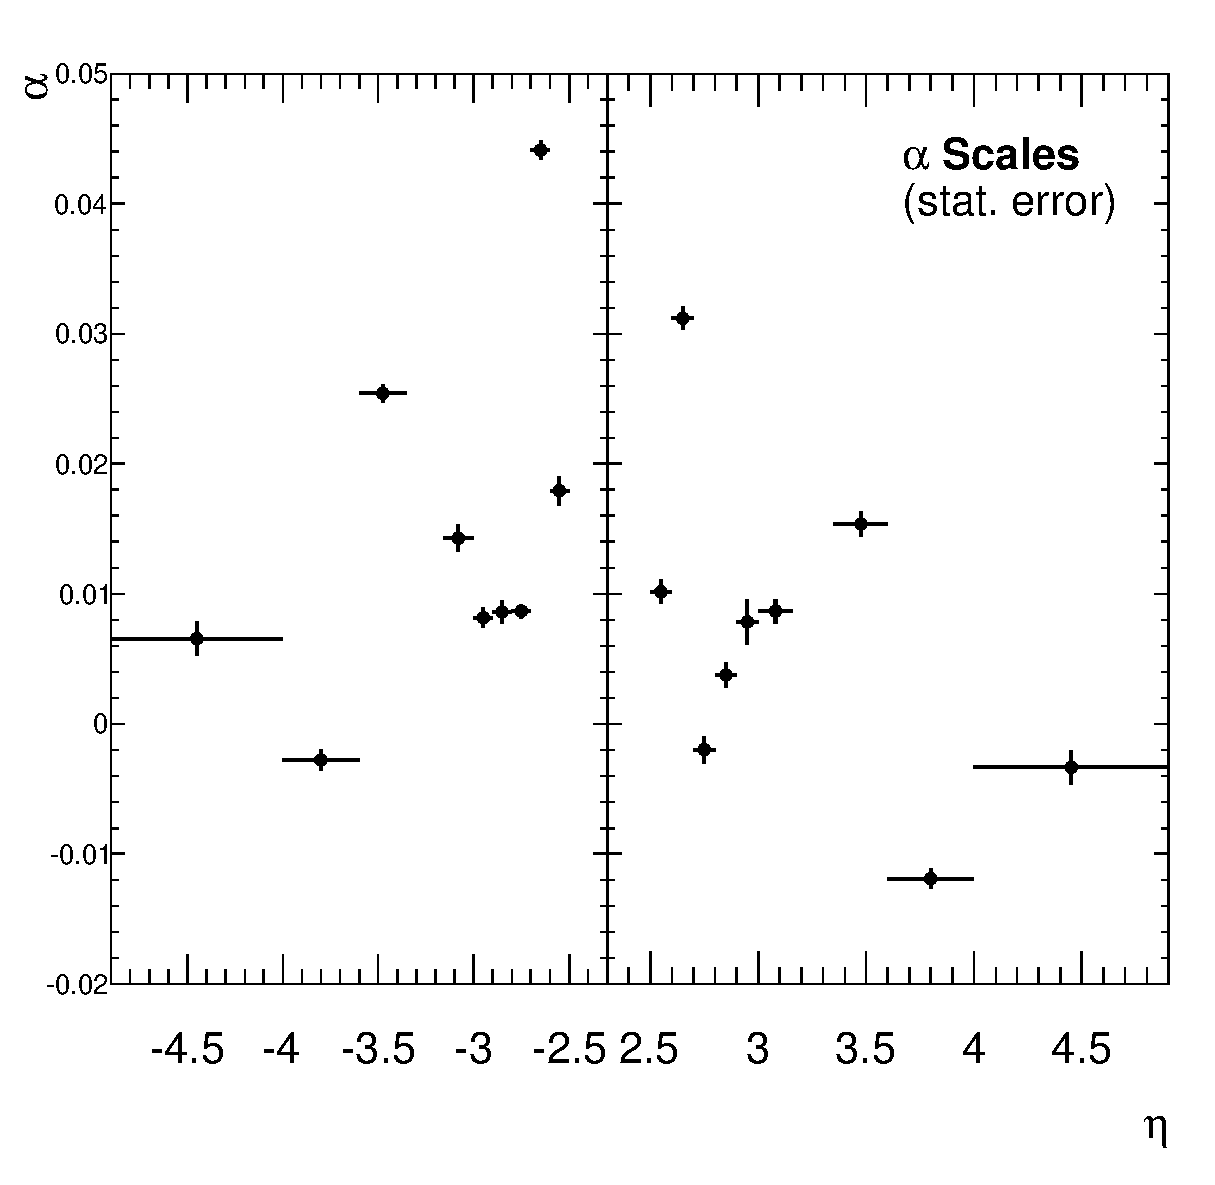
\includegraphics[width=1.\textwidth]{plots/alpha_stat}
        \captionsetup{format=plain}
        \caption{Kalibrations-Faktoren der Energieskala für die verschiedenen
            Bereiche des Kalorimeters (nur statistische Unsicherheiten)}
        \label{fig:alpha_stat}
    \end{minipage}
    \hfill
    \begin{minipage}{0.48\textwidth}
        \centering
        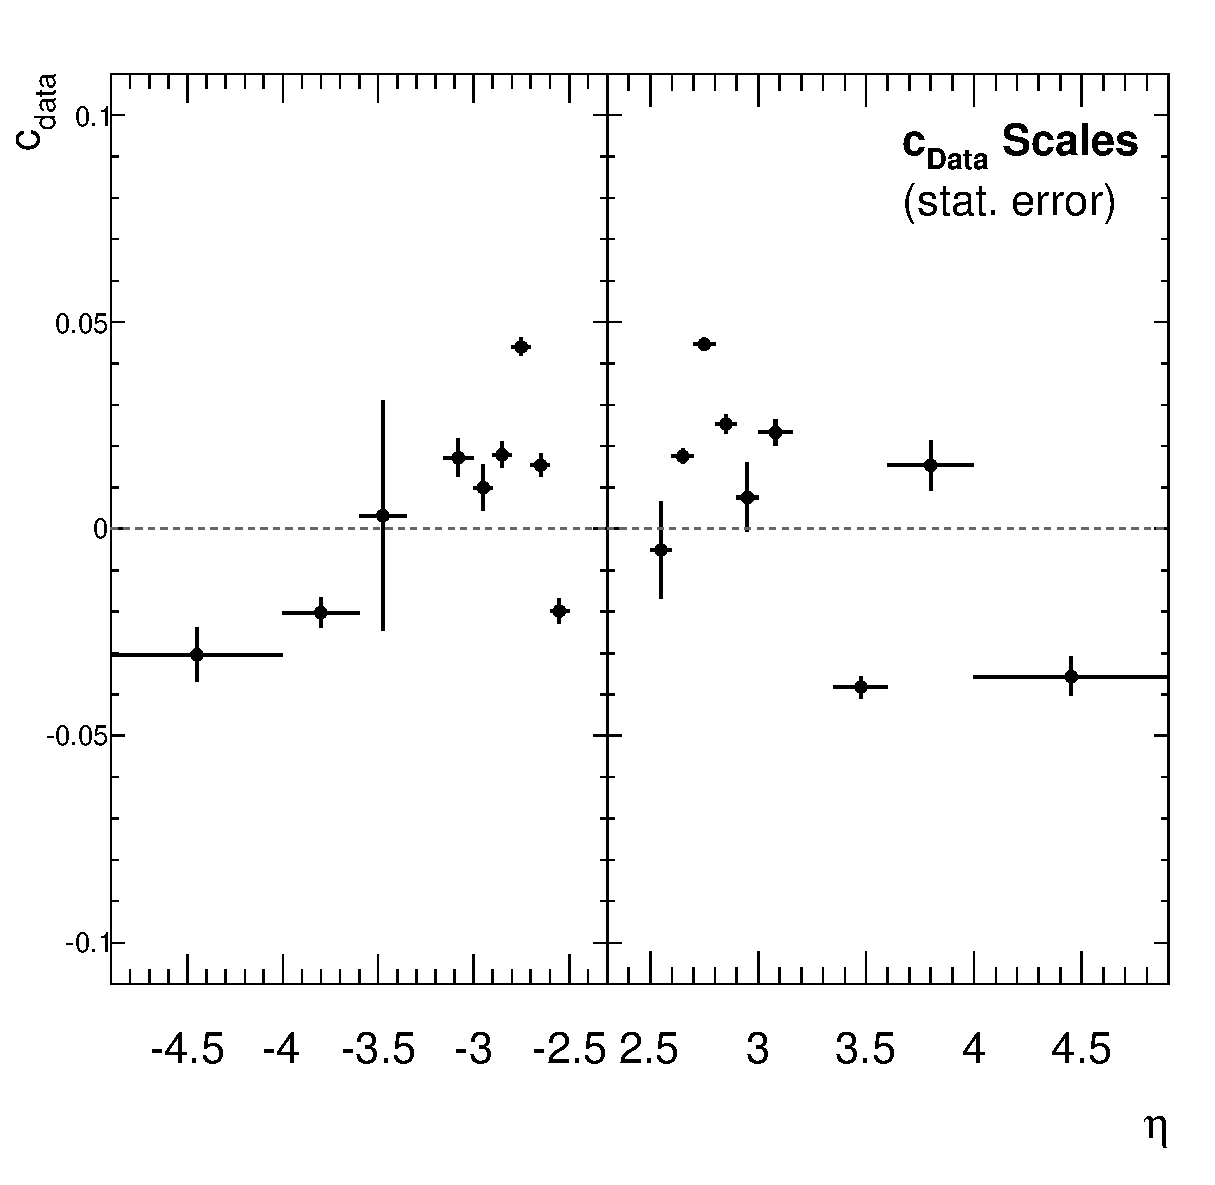
\includegraphics[width=1.\textwidth]{plots/cdata_stat}
        \captionsetup{format=plain}
        \caption{Kalibrations-Faktoren der Auflösung für die verschiedenen
            Bereiche des Kalorimeters (nur statistische Unsicherheiten)}
        \label{fig:cdata_stat}
    \end{minipage}
\end{figure}

Man erkennt, dass die Korrekturen im Bereich weniger Prozent liegen und
zumindest eine schwache Symmetrie in der Struktur der Verteilung im negativen
und positiven Pseudorapiditäts-Bereich aufweisen.

Diese Faktoren werden nun verwendet, um in der zweiten Iteration die
Energieskala der Vorwärts-Elektronen in den Daten zu korrigieren
(\textit{Vorbereitung II}) und anschließend die Extraktion der
Kalibrations-Faktoren der Auflösung (\textit{Extraktion II}) vorzunehmen.
Dabei beobachtet man in einigen Bereichen des Kalorimeters, dass der Radikand
in Gleichung (\ref{eq:constant_terms}) negative Werte annimmt, sodass die
Wurzel auf den reellen Zahlen nicht mehr definiert ist. Dieser Fall tritt immer
dann auf, wenn die Auflösung in den Daten besser ist, als die Simulation dies
beschreibt.
\begin{equation}
    \sigma_\text{(data)} < \sigma_\text{(MC)}
    \label{eq:resolution}
\end{equation}

Die resultierenden Werte für diese Faktoren $c_i$ sind in Abbildung
\ref{fig:cdata_stat} zu sehen und ebenfalls mit statistischen Unsicherheiten
aufgetragen. Für den oben beschriebenen Fall (\ref{eq:resolution}) wurde hier
das Vorzeichen des Radikanden vor die Wurzel gezogen (negative $c_i$), um ein
Maß für den Unterschied der Auflösung in Daten und Simulation zu gewinnen. Auch
für die Kalibrations-Faktoren der Auflösung liegen die Korrekturen im
Prozent-Bereich und zeigen in ihrer Struktur eine gewisse Symmetrie.

In dieser zweiten Iteration ist es zudem möglich eine Konsistenz-Prüfung der
zuvor extrahierten Kalibrations-Faktoren $\alpha_i$ durchzuführen. Da die
Energieskala der Vorwärts-Elektronen in \textit{Vorbereitung II} durch diese
korrigiert wurden, müsste der Versuch einer erneuten Extraktion zu
verschwindenen Kalibrations-Faktoren führen. Abbildung \ref{fig:alpha_2nd}
zeigt diesen Versuch der erneuten Extraktion der Kalibrations-Faktoren für die
Energie-Skala\footnote{Um Verwechslungen auszuschließen mit $\alpha'_i$
bezeichnet}.

\begin{figure}
    \centering
    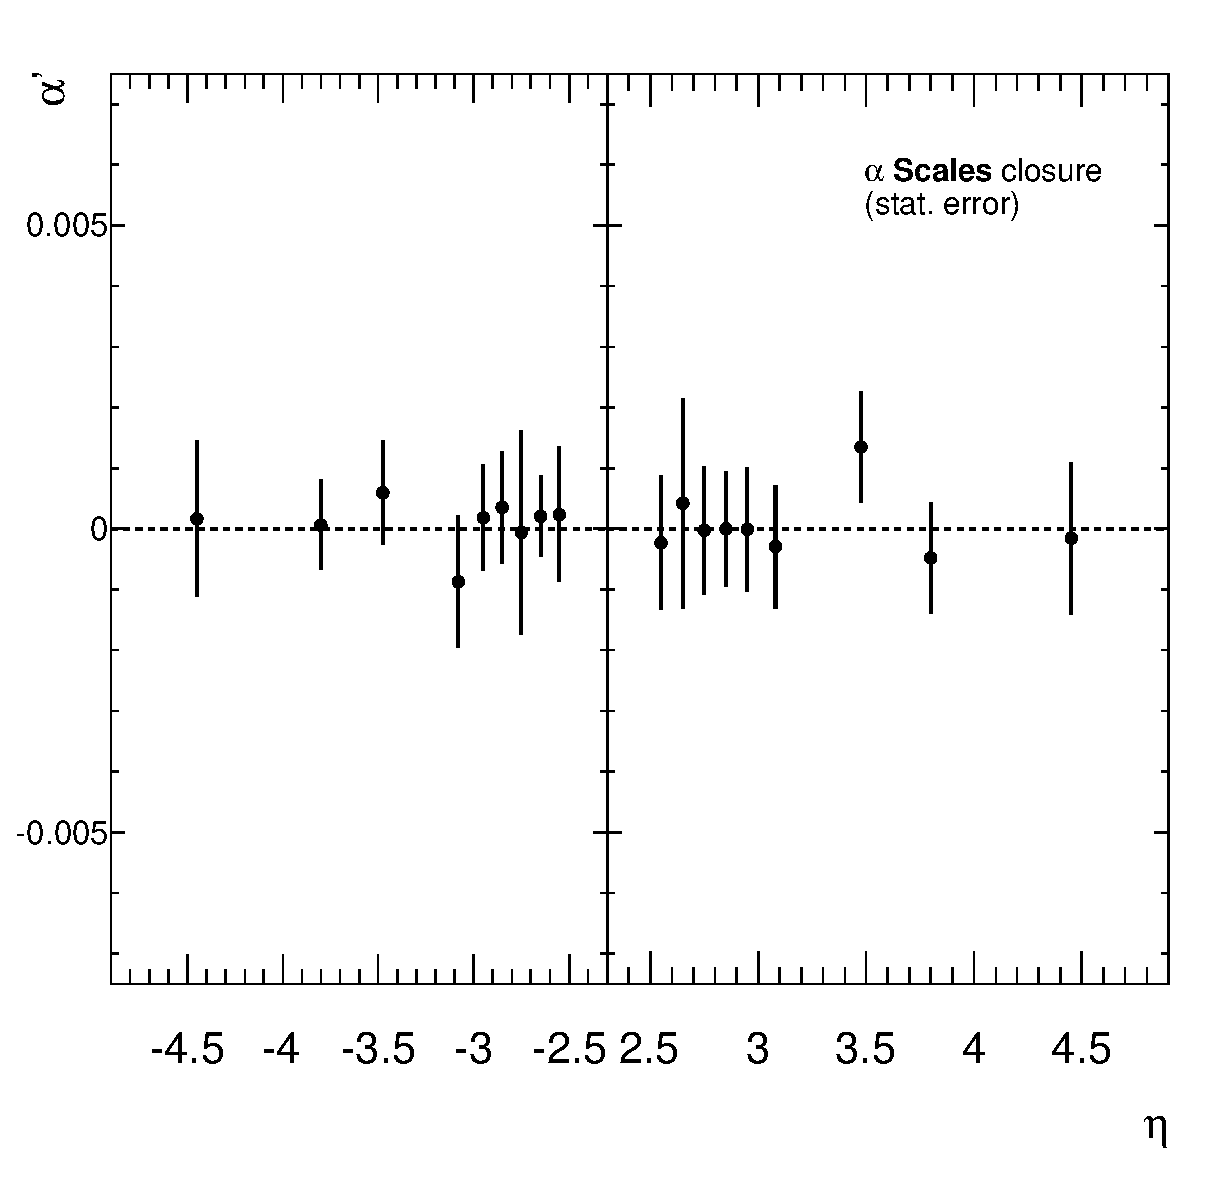
\includegraphics[width=0.6\textwidth]{plots/alpha_2nd}
    \caption[Konsistenz-Prüfung der extrahierten Kalibrations-Faktoren
        $\alpha_i$ der Energieskala]
        {Konsistenz-Prüfung der extrahierten Kalibrations-Faktoren
        $\alpha_i$ der Energieskala. Nach Korrektur der Energieskalen durch die
        $\alpha_i$ wird erneut versucht Kalibrations-Faktoren $\alpha'_i$ zu
        bestimmen}
    \label{fig:alpha_2nd}
\end{figure}

Wie sich sich zeigt sind mit einer Ausnahme alle Faktoren $\alpha'_i$ innerhalb
ihrer statistischen Unsicherheiten mit Null verträglich, was für die Konsistenz
der ermitteln Kalibrations-Faktoren bestätigt.



\subsection{Systematische Unsicherheiten}
\label{energy_calibration:systematics}
Die Bestimmung der Kalibrations-Faktoren für Energie und Auflösung basiert auf
gewissen Annahmen und Vorraussetzungen wie bespielsweise die vorangegangene
Kalibration der Zentral-Elektronen (vgl. Abschnitt
\ref{energy_calibration:definitionen_und_annahmen}).
Hierdurch werden unter Umständen systematische Effekte eingeführt, die sich auf
die zu bestimmenden Faktoren auswirken. Zu deren Studium variiert man die
eingehenden Größen einzeln innerhalb ihrer Unsicherheit und wiederholt die
obige Extraktions-Prozedur für jede dieser geänderten Konfigurationen separat.
Die mögliche Abweichung von den zuvor in
\ref{energy_calibration:extraction_energy_scales} bestimmten Werten $\alpha_i$
und $c_i$ ist dann ein Maß für den Einfluss der variierten Größe und induziert
somit zusätzliche systematische Unsicherheiten.

Folgende Zusammenstellung zeigt die untersuchten systematischen Einflüsse und
deren Variation im Sinne der oben beschriebenen Änderungen der Konfiguration.

\begin{description}
    \item[Kalibration der Zentral-Elektronen:]
        Der offensichtlichste Effekt ist der Einfluss der Kalibration der
        Elektronen im Zentral-Bereich. Da diese in
        \ref{energy_calibration:definitionen_und_annahmen} als perfekt
        kalibriert angenommen wurden hat deren Unsicherheit direkten Einfluss
        auf die Extraktion der Kakibrations-Faktoren.
        
        Das zur Anwendung der Korrekturen von ATLAS bereitgestellte
        Software-Paket\footnote{siehe Abschnit \ref{},
        \textit{EnergyRescalerUpgrade}} bietet die Möglichkeit systematische
        Variationen der Kalibrations-Faktoren für die Zentral-Elektronen
        durchzuführen. Diese werden, entsprechend der internen Empfehlungen zu
        diesem Paket, separat durchgeführt die resultierenden Abweichungen
        später quadratisch aufsummiert.

    \item[Skalenfaktoren der Rekonstruktions-Effizienzen:]
        Die Effizienzen für die Rekonstruktion von Elektronen werden in der
        Simulation nachträglich durch Skalenfaktoren korrigiert (siehe hierzu
        Abschnitt \ref{}). Die Bestimmung dieser Skalenfaktoren unterliegt
        jedoch ebenfalls gewissen Unsicherheiten, welche Einfluss auf die
        extrahierten Kalibrations-Faktoren nehmen.

        Auch hier ist es softwareseitig möglich, die Variation der
        Skalenfaktoren innerhalb ihrer Unsicherheiten unabhängig voneinander
        durchzuführen.

    \item[Massenfenster:]
        Die spezielle Wahl des Massenfensters, in dem die Spektren der
        invarianten Masse betrachtet und die Kurvenanpassungen durchgeführt
        werden, impliziert durch die Hinzuname bzw. das Ausschließen von
        Datenpunkten eine gewisse Variation der Kalibrations-Konstaten.

        Aus diesem Grund wird neben dem Standard-Massenfenster, auch ein
        vergrößertes Massenfenster betrachtet:
        \[
            70 \GeV < m_{ee} < 110 \GeV
        \]
        %Ein weitere Variation mit einem gegenüber des Standards verkleinerten
        %Massenfenster wurde untersucht, stellte sich allerdings als wenig
        %sinnvoll heraus, da 

    \item[Untergrund-Modell:]
        Wie in \ref{energy_calibration:extraktionsmethode} beschrieben wird der
        in den Daten nach Selektion verbleibende Untergrund mit einer
        Exponentialfunktion abgeschätzt. Obwohl diese Wahl physikalisch
        motiviert und sinnvoll ist, so sie auch auf eine andere Funktion fallen
        können, die ebenso plausibel den Untergrund modelliert.

        Als alternative Verteilung wird deshalb ein Potenzgesetz der Form
        \[
            f_\text{bkg}(m_{ee}) \sim\;\frac{a}{m_{ee}^4}
        \]
        gewählt und so der Einfluss des Untergundmodells ermittelt.

    \item[Parameter der kinematischen Akzeptanz:]
        In Abschnitt
        \ref{energy_calibration:erweiterung_der_modelle_und_prozedur} wurde die
        Erweiterung der analytischen Modelle durch die kinematische Akzeptanz
        eingeführt, 

\end{description}





%______________________________________________________________________________
%                                                       Ergebnisse und Ausblick 
%
\section{Ergebnisse und Ausblick}
\label{energy_calibration:ergebnisse_und_ausblick}
\begin{itemize}
    \item Zusammenfassung
    \item Diskussion ( Dominiert von Zentral-Skalen, Modell-Probleme )
    \item Verbesserungen ( Neue Zentral-Skalen, Template-Ansatz )
\end{itemize}


